\chapter{Results}\label{res}

The following chapter summarizes the results obtained by overlapping simple closed form template models with each of the 200 waveforms present in the catalogs introduced in section \ref{NR}. Furthermore, the parameters that maximize the SNR recovery for a given model will be extracted for different purposes:

\begin{enumerate}
\item Given a finite monochromatic model with constant amplitude, find out which BNS postmerger waveform could be detectable at 100MPc using the matched filtering algorithm.

\item In the case of detectable postmerger sources, examine how well the model recovers waveform features like its main frequency and duration.

\item Check whether modeling the postmerger's first amplitude minimum (see figure \ref{}) with zero crossing amplitude envelopes can improve the SNR and parameter recovery for some waveforms in the catalog.

\end{enumerate}


To complete this task, the code described in section \ref{} will be generalized for j=220 waveforms $h^j$ and templates with n-free parameters $q$. Since one can map a unique template $q$ to each point in the parameter space represented by the n-tuple $(a_1,...,a_n)$, template models will from now on be interpreted in geometrical terms as an n-dimensional object called \textit{template bank}. 

\begin{equation}\label{ndim}
q_{_{a_1,...,a_n}}(t)
\end{equation}

Such n-dimensional template bank will be used to compute its inner products \ref{} with each singal $h^j$, such that the SNR in an n-dimensional grid can be written as 

\begin{equation}\label{pul}
\rho^j_{_{_{a_1,...,a_n}}} = \frac{\langle h^j, q_{_{_{a_1,...,a_n}}}\cdot e^{i(2\pi \tau+\phi)}\rangle \bigg\rvert_{\phi =\phi_{opt},\tau =\tau_{max}}}{\sqrt{\langle  q_{_{_{a_1,...,a_n}}},q_{_{_{a_1,...,a_n}}} \rangle}}
\end{equation}


Of which the global maximum, and its location in parameter space $a_{1_{best}},...,a_{n_{best}}$ will be extracted 

\begin{equation}
\rho_{max} = \rho_{_{a_{1_{best}},...,a_{n_{best}},\phi_{opt},\tau_{max}}}
\end{equation}

Where $\phi_{opt},\tau_{max}$ are the optimal phase and timeshift extracted to reconstruct the signal in the time domain as shown in figure \ref{fig:7}. 

During the development of this thesis, a Python code that provides an interface to compute waveform strain, generate simple template banks and runs the matched filtering algorithm iteratively on one or more catalogs of NR waveforms was implemented. The following flowchart shows its infrastructure and outlines the technical difficulties encountered when dealing with sets of waveforms that use different file formats, resolutions, unit systems for physical observables, and missing metadata.


\newpage


\begin{sidewaysfigure}[hbt!]
\begin{center}
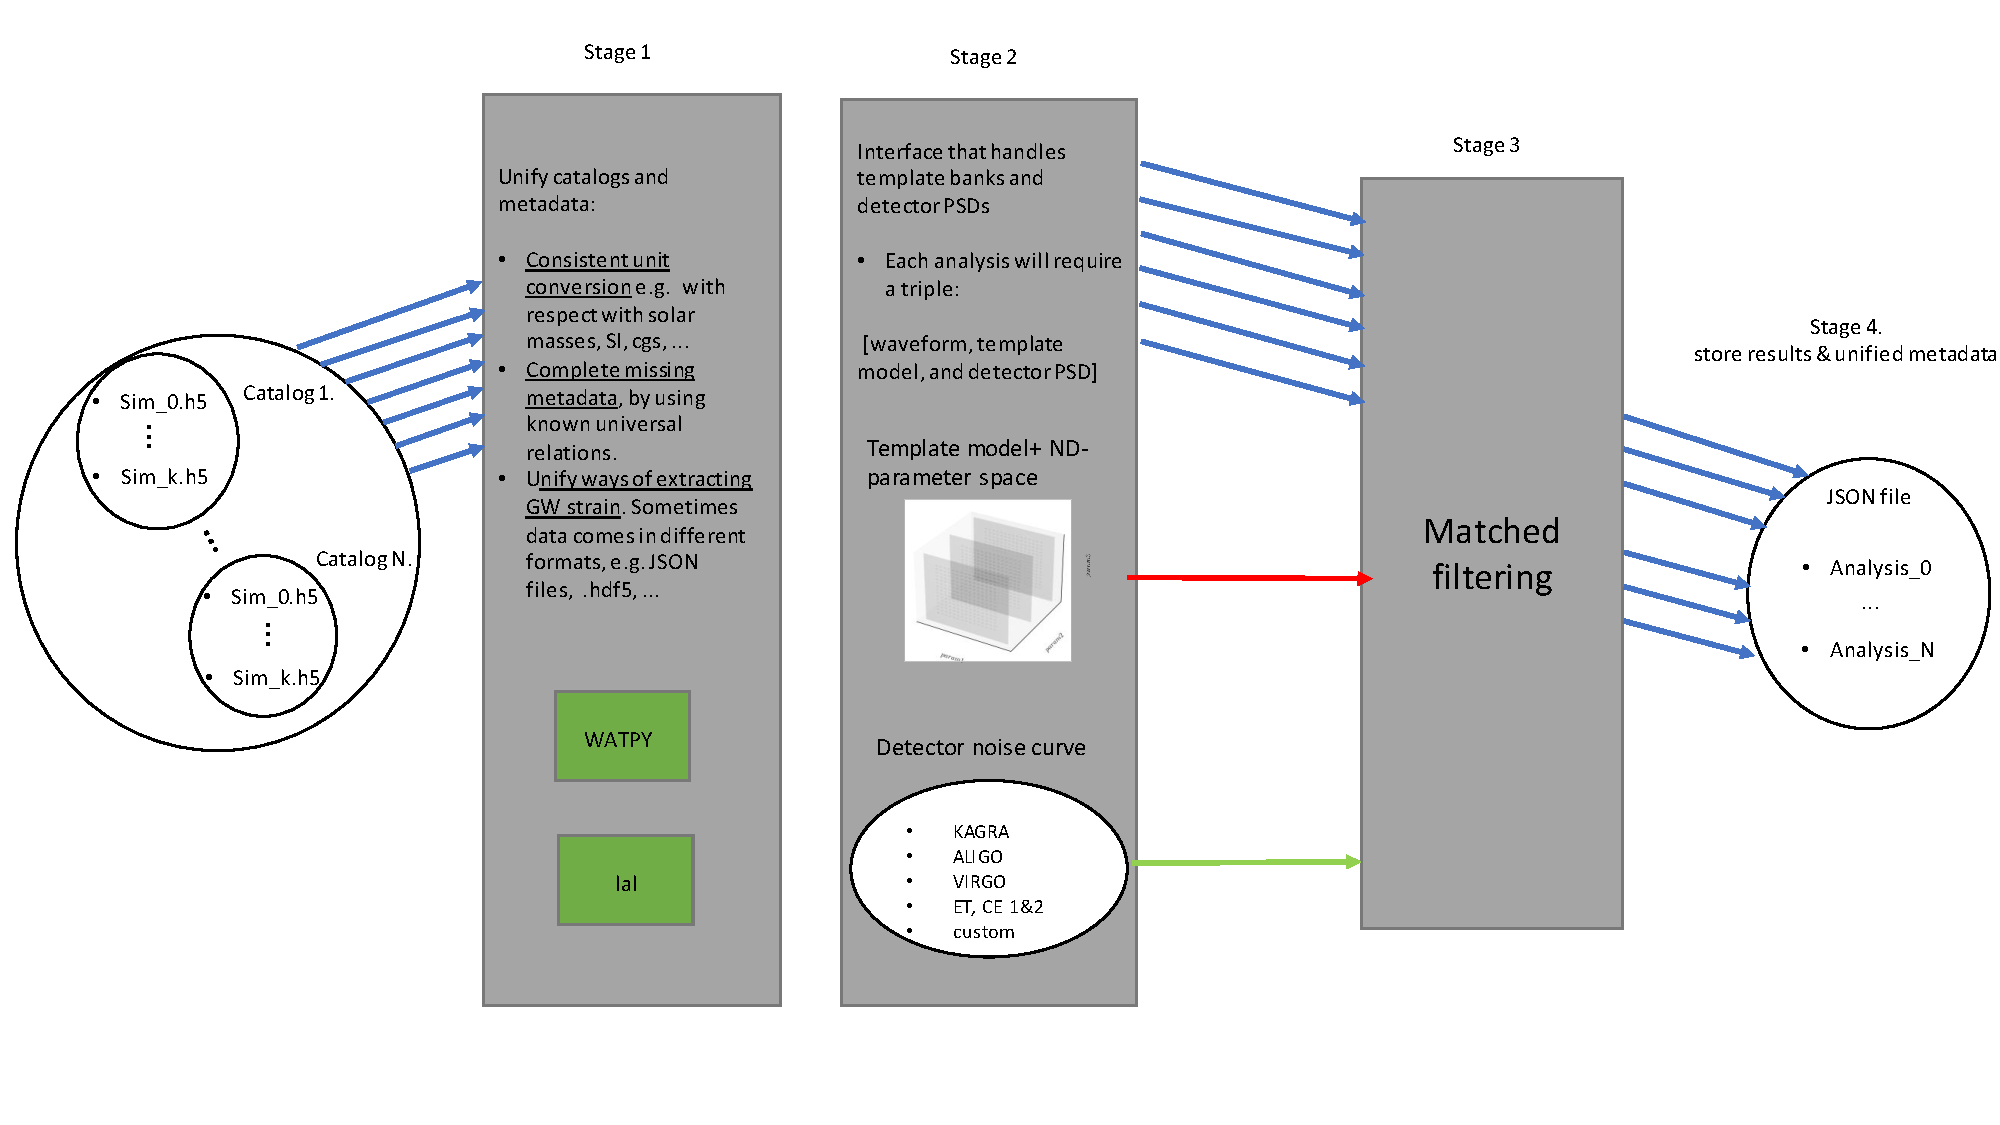
\includegraphics[width=\textwidth, angle=0]{images/cat_search.pdf}
\captionsetup{width=0.8\textwidth}
\caption{Flowchart of matched filter code for NR waveform catalogs}
\caption*{This flowchart contains the schematics of the matched filtering code for NR waveform catalogs\cite{}. It is divided in 4 stages, of which only stage 3 employs equation \ref{pul}. Stages 1 and 2 are depict the waveform extraction done through python packages like WATPY and LAL; template bank generation and conditioning of detector sensitivity curves; and stage 4 for results and metadata storage.}
\label{fig:19}
\end{center}
\end{sidewaysfigure}

\FloatBarrier


\section{The 2-dimensional finite monochromatic model}\label{2dsearch}

The following section will consider a template model that only accounts for the most dominant frequency and duration of a BNS postmerger GW. Hence, it will be constructed by using a sinusoidal wave with constant amplitude and frequency, and a rectangular window to define its finite duration 

%\begin{equation}\label{eq:19}
%q_{_{_{A, f, \phi_0, t_{0}, d}}}(t) =A \cdot sin(2\pi f t + \phi_0) \cdot \Pi_{t_{0},t_{0} + d}(t)=
%\begin{cases} 
%      0 & t<t_{0} \\
%      A \cdot sin(2\pi f t + \phi_0) & t_{0} \leq t\leq t_{0}+d \\
%      0 & t>t_{0}+d
%   \end{cases}
%\end{equation}

\begin{equation}\label{eq:19}
q_{_{_{A, f, \phi_0, t_{0}, d}}}(t) =A \cdot sin(2\pi f t + \phi_0) \cdot \Pi_{t_{0},t_{0} + d}(t)
\end{equation}


\begin{equation}\label{eq:18}
\Pi_{_{_{a,b}}}(t) = \theta(t-a)-\theta(t-b) = 
\begin{cases} 
      0 & a<t \\
      1 & a \leq t\leq b \\
      0 & b>t
   \end{cases}
\end{equation}

Where $t_0$ is wave starting time, $t_0+d$ and $f$ its duration and frequency , and $A$ and $\phi$ its amplitude and phase.


As seen in section \ref{}, matched filtering algorithm allows to find the optimal values for amplitude, phase and timeshift $A_{opt}$, $\phi_{opt}$ and $t_{0_{opt}}$, such that the template model \ref{eq:19}, can be written as

\begin{equation}\label{eq:20}
q_{_{_{f,d}}}(t) =
\begin{cases} 
      0 & t<t_{0_{opt}} \\
      A_{opt} \cdot sin(2\pi f t + \phi_{0_{opt}}) & t_{0_{opt}} \leq t\leq t_{0_{opt}}+d \\
      0 & t>t_{0_{opt}}+d
   \end{cases}
%\label{eq_uk}.
\end{equation}

The recovered SNR equation \ref{pul}, can be written in terms of the 2-dimensional bank of templates \ref{eq:20}

\begin{equation}\label{eq:21}
\rho_{_{_{f,d}}} = \frac{\langle h, q_{_{_{f,d}}}\cdot e^{i(2\pi \tau+\phi)}\rangle \bigg\rvert_{\phi =\phi_{opt},\tau =\tau_{max}}}{\sqrt{\langle  q_{_{_{f,d}}},q_{_{_{f,d}}} \rangle}}
\end{equation}


For the sake of simplicity, in this thesis template banks will be constructed in a uniform rectangular grid of 200 by 200 points, where the $f$-dimension varies from 500 to 3500 Hz, and the duration dimension varies between 0.1 milliseconds and $1.5 \cdot d_{postm}$. 

\begin{figure}[!htb]
\centering
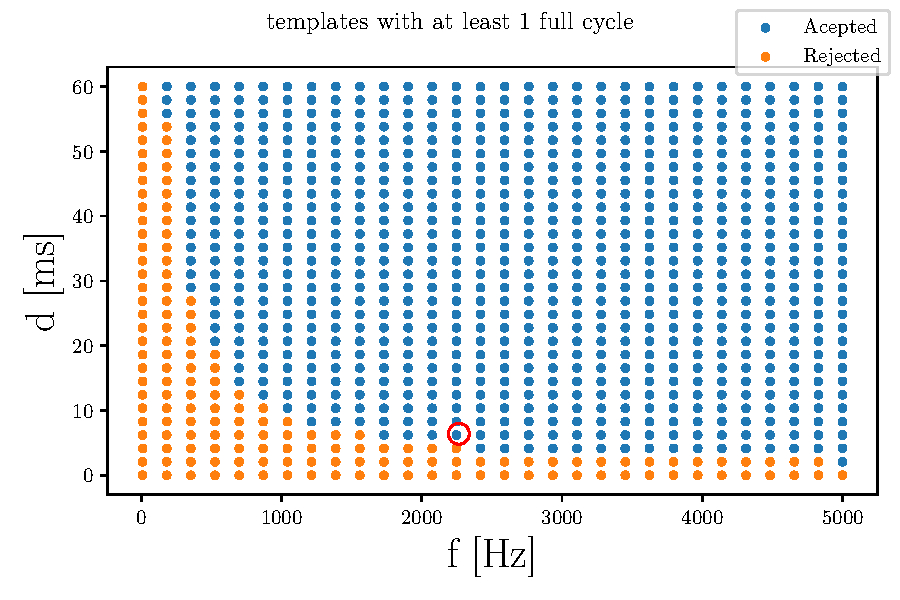
\includegraphics[scale=0.55]{images/Data_analysis/results/param_space.pdf}
\captionsetup{width=0.8\textwidth}
\caption{The parameter space of a monochromatic wave}
\caption*{This figure shows how the parameter space of a monochromatic wave. A mask is applied to discard combinations $(f,d)$ that generate templates with less than 1 wavelenght.The red circle shows the template used in figure \ref{}}
\end{figure}
\FloatBarrier

%However, notice that there are different algorithms that address the problem of building template banks optimally, which is beyond the scope of what is presented here\cite{Allen_2021}.

Subsequently, the recovered SNR, normalized by the optimal SNR \ref{sopt}, will be computed at each point of the grid and will be represented as a the third dimension using colormaps. 


The following figure, shows how a \textit{Non-spinning equal mass BNS systems} may generate a signal with slow amplitude and frequency variations. Overlapping such waveform against  the template model \ref{} produces a colormap where 2 main regions show SNR peaks: the first between 1.5-2 kHz below 5 ms and the second between 2-2.5 kHz with a peak at 15ms. 

\begin{figure}[!htbp]
\begin{center}
\begin{minipage}[t]{0.5\linewidth}
\vspace{0pt}
%\raggedleft
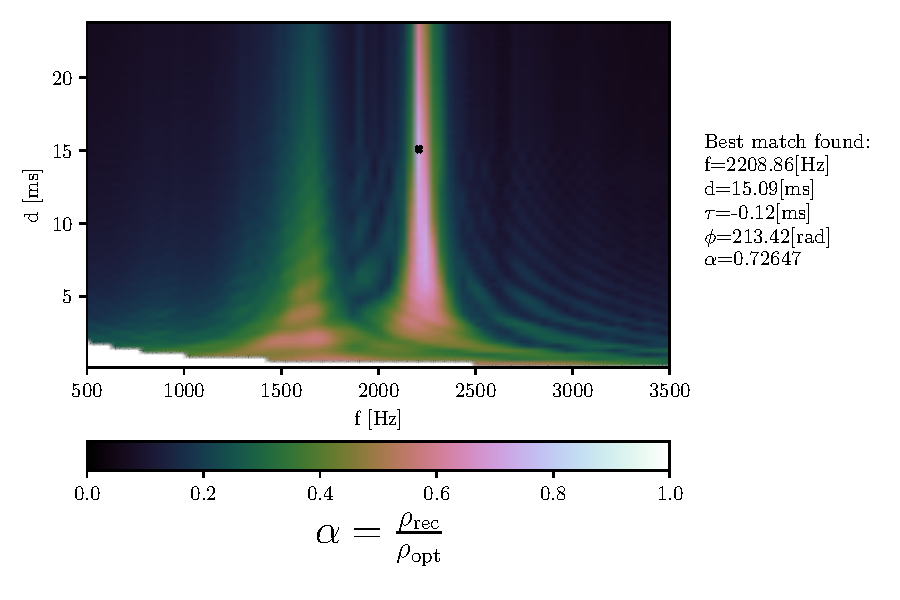
\includegraphics[scale=0.6,trim={2mm 0 35mm 0},clip]{images/Data_analysis/results/2D_grid_1.pdf}
\end{minipage}%
\begin{minipage}[t]{0.5\linewidth}
\vspace{20pt}
%\raggedright
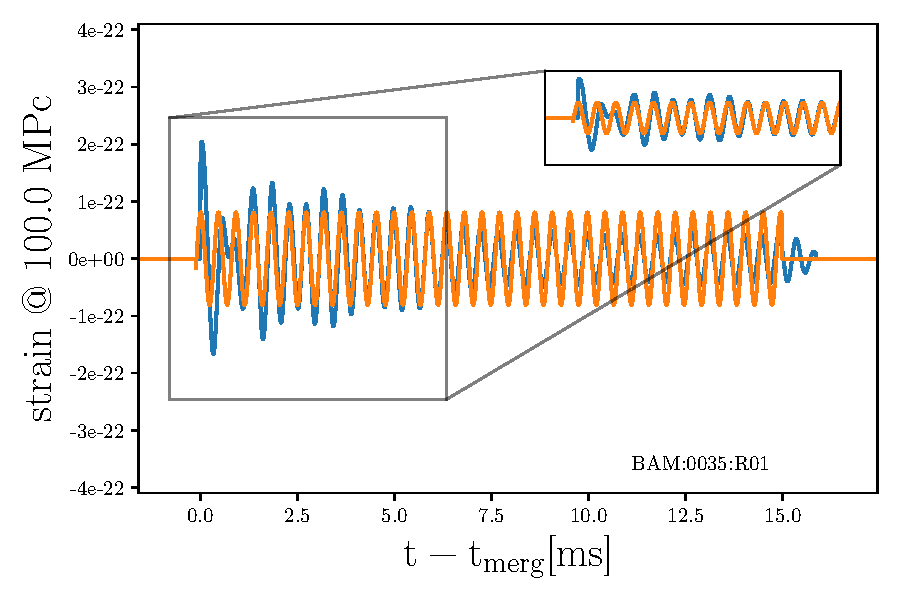
\includegraphics[scale=0.45]{images/Data_analysis/results/2D_grid_2.pdf}
\end{minipage}
\captionsetup{width=0.8\textwidth}
\caption{Equal mass BNS waveform and its best monochromatic match}
\caption*{This plot shows the recovered SNR \ref{} for the waveform BAM:0035:R01 of the CoRe BNS catalog \cite{}(see figure\ref{} to read the BNS poperties) and the template model \ref{}. The best matching parameters are $f=Hz$, $d=ms$.}
\end{center}
\end{figure}

\FloatBarrier

%In this example, the postmeger tail has a high amplitude and a slowly varying frequency which helps the monochromatic model \ref{} recover a long duration without losing SNR due to misalignments with the waveform. 

Below a few other example waveforms will be overlapped against the template model \ref{} to depict how the matched filtering algorithm can, for other more complex BNS postmerger signals, recover more SNR with short monochromatic segments instead.
 

\textit{High mass ratio BNS systems}, i.e. $q=m_1/m_2>1.6$ may show also 2 regions with excess SNR recovery. However the low frequency-low duration region of parameter space dominates.

\begin{figure}[!htbp]
\begin{center}
\begin{minipage}[t]{0.5\linewidth}
\vspace{0pt}
%\raggedleft
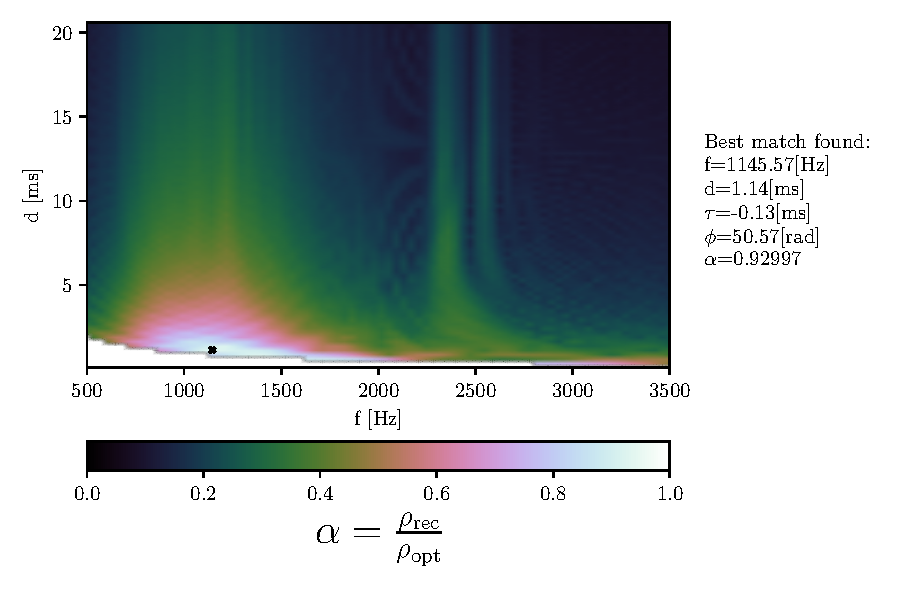
\includegraphics[scale=0.6,trim={2mm 0 35mm 0},clip]{images/Data_analysis/results/2D_grid_3.pdf}
\end{minipage}%
\begin{minipage}[t]{0.5\linewidth}
\vspace{20pt}
%\raggedright
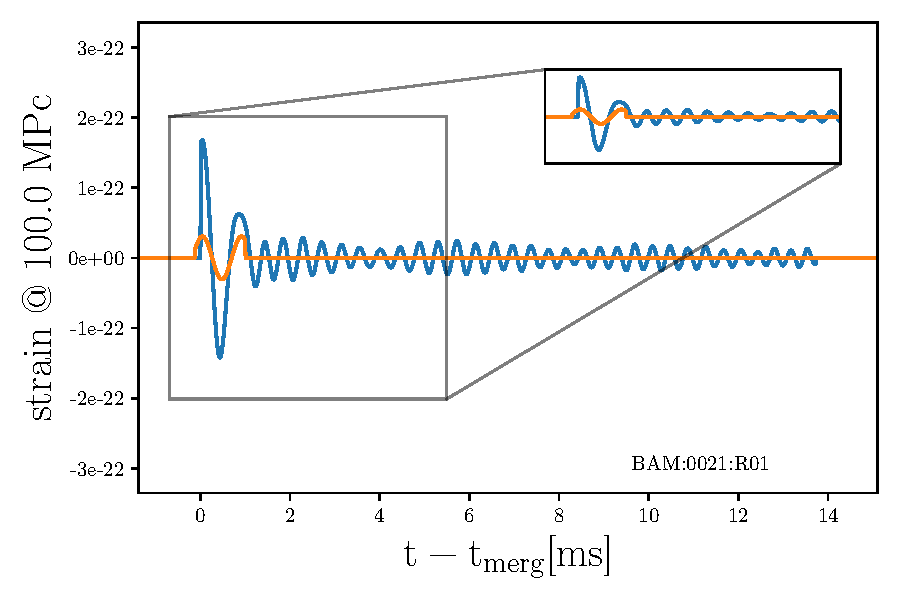
\includegraphics[scale=0.45]{images/Data_analysis/results/2D_grid_4.pdf}
\end{minipage}
\captionsetup{width=0.8\textwidth}
\caption{High mass ratio BNS waveform and its best monochromatic match}
\caption*{This plot shows the recovered SNR \ref{} for the waveform BAM:0021:R01 of the CoRe BNS catalog \cite{}(see figure\ref{} to read the BNS poperties) and the template model \ref{}. The best matching parameters are $f=Hz$, $d=ms$.}
\end{center}
\end{figure}

\FloatBarrier


\newpage

\textit{Spinning BNS systems} i.e. $\chi_{eff}>0.2$(see equation \ref{}) have a more complex frequency evolution. The colormap shows 2 regions of SNR excess: a wide one ranging from 1-2.5 kHz and duration below 5ms, and the other between 3-3.5 kHz with a peak duration around half waveform's duration $d_{postm}$. Notice that both regions have similar amounts of SNR recovery, so even though this example waveform prefers a long high frequency monochromatic segment, in some other cases it may be a short low frequency one.

\begin{figure}[!htbp]
\begin{center}
\begin{minipage}[t]{0.5\linewidth}
\vspace{0pt}
%\raggedleft
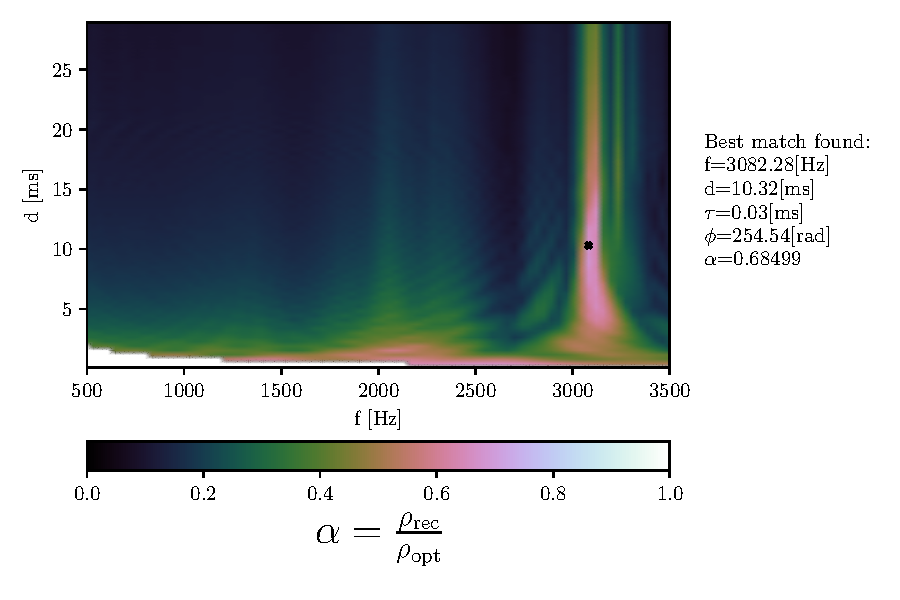
\includegraphics[scale=0.6,trim={2mm 0 35mm 0},clip]{images/Data_analysis/results/2D_grid_5.pdf}
\end{minipage}%
\begin{minipage}[t]{0.5\linewidth}
\vspace{20pt}
%\raggedright
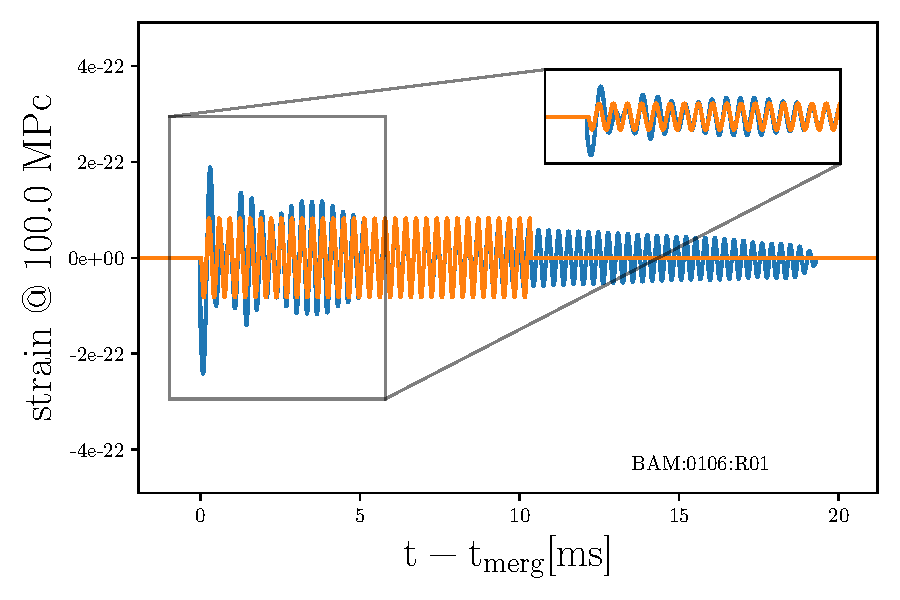
\includegraphics[scale=0.45]{images/Data_analysis/results/2D_grid_6.pdf}
\end{minipage}
\captionsetup{width=0.8\textwidth}
\caption{Spinning BNS waveform and its best monochromatic match}
\caption*{This plot shows the recovered SNR \ref{} for the waveform BAM:0106:R01 of the CoRe BNS catalog \cite{}(see figure\ref{} to read the BNS poperties) and the template model \ref{}. The best matching parameters are $f=Hz$, $d=ms$.}
\end{center}
\end{figure}

\FloatBarrier



\textit{Heavy BNS systems} i.e. $\delta=\frac{M_g}{M_{TOV}}>1.6$ may generate very short waveforms that contain at least one full high-frequency cycle(around 3 kHz) that can be easily fitted with a monochromatic wave.

\begin{figure}[!htbp]
\begin{center}
\begin{minipage}[t]{0.5\linewidth}
\vspace{0pt}
%\raggedleft
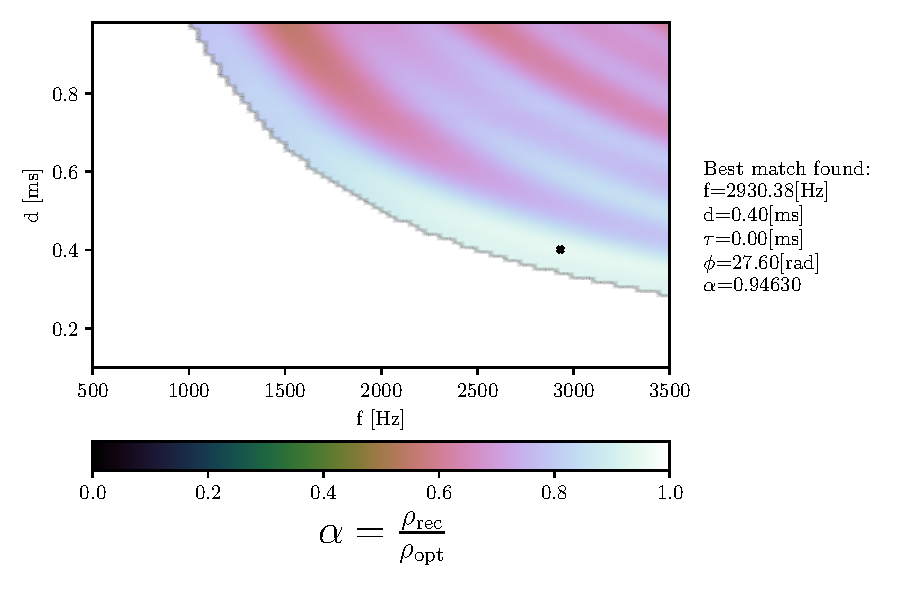
\includegraphics[scale=0.6,trim={2mm 0 35mm 0},clip]{images/Data_analysis/results/2D_grid_7.pdf}
\end{minipage}%
\begin{minipage}[t]{0.5\linewidth}
\vspace{20pt}
%\raggedright
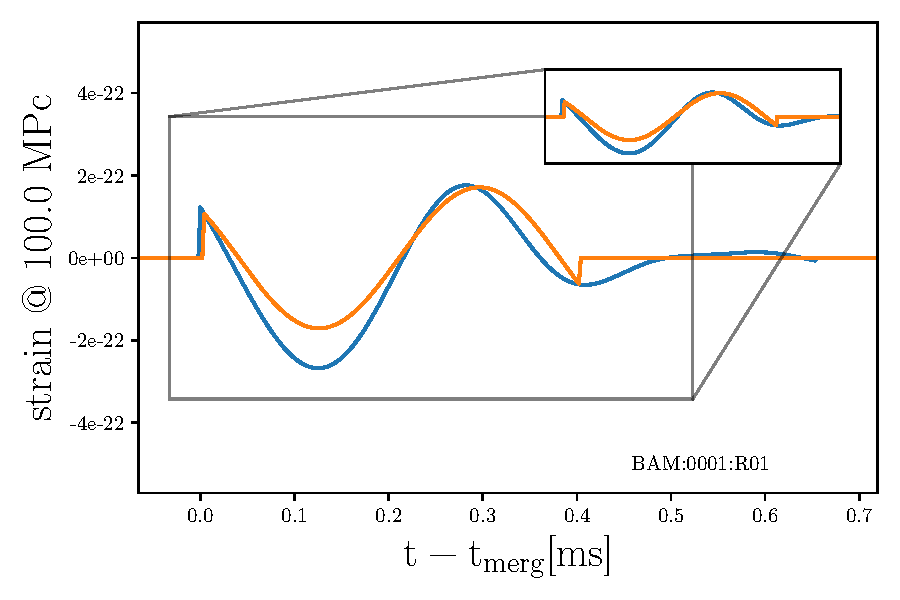
\includegraphics[scale=0.45]{images/Data_analysis/results/2D_grid_8.pdf}
\end{minipage}
\captionsetup{width=0.8\textwidth}
\caption{Spinning BNS waveform and its best monochromatic match}
\caption*{This plot shows the recovered SNR \ref{} for the waveform BAM:0001:R01 of the CoRe BNS catalog \cite{}(see figure\ref{} to read the BNS poperties) and the template model \ref{}. The best matching parameters are $f=Hz$, $d=ms$.}
\end{center}
\end{figure}

\FloatBarrier
 

\newpage
\textit{Highly eccentric BNS systems} i.e. $e>0.4$, show a wide structure on the low-frequency side that dominates the colormap, resulting in short best matches, similarly to high mass ratio waveforms


\begin{figure}[!htbp]
\begin{center}
\begin{minipage}[t]{0.5\linewidth}
\vspace{0pt}
%\raggedleft
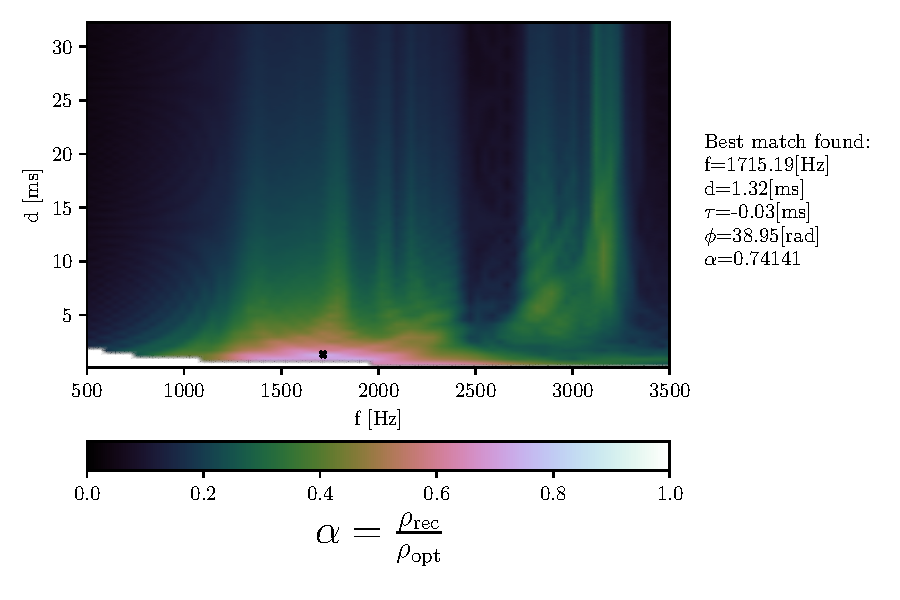
\includegraphics[scale=0.6,trim={2mm 0 35mm 0},clip]{images/Data_analysis/results/2D_grid_9.pdf}
\end{minipage}%
\begin{minipage}[t]{0.5\linewidth}
\vspace{20pt}
%\raggedright
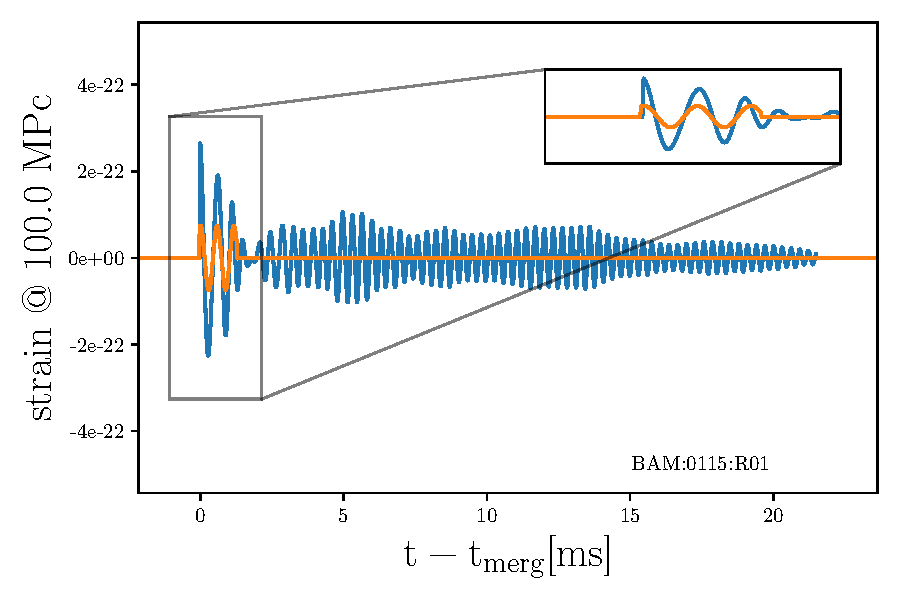
\includegraphics[scale=0.45]{images/Data_analysis/results/2D_grid_10.pdf}
\end{minipage}
\captionsetup{width=0.8\textwidth}
\caption{Spinning BNS waveform and its best monochromatic match}
\caption*{This plot shows the recovered SNR \ref{} for the waveform BAM:0115:R01 of the CoRe BNS catalog \cite{}(see figure\ref{} to read the BNS poperties) and the template model \ref{}. The best matching parameters are $f=Hz$, $d=ms$.}
\end{center}
\end{figure}

\FloatBarrier


\textit{Equal mass BNS systems} with Viscuous hydrodynamics generate waveforms with a stonger amplitude modulation as compared to the example shown in figure \ref{}. However, such effects do not change significantly change the colormaps.

\begin{figure}[!htbp]
\begin{center}
\begin{minipage}[t]{0.5\linewidth}
\vspace{0pt}
%\raggedleft
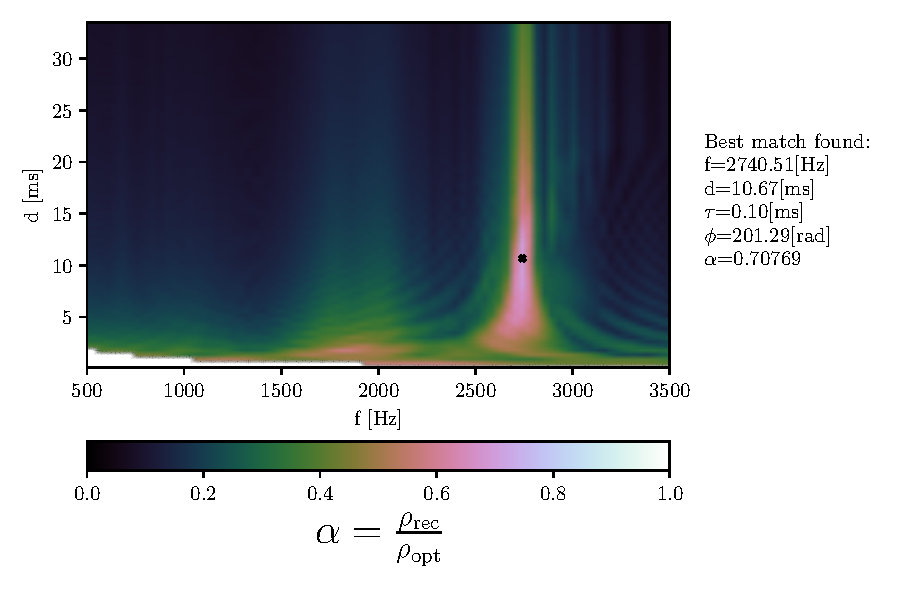
\includegraphics[scale=0.6,trim={2mm 0 35mm 0},clip]{images/Data_analysis/results/2D_grid_11.pdf}
\end{minipage}%
\begin{minipage}[t]{0.5\linewidth}
\vspace{20pt}
%\raggedright
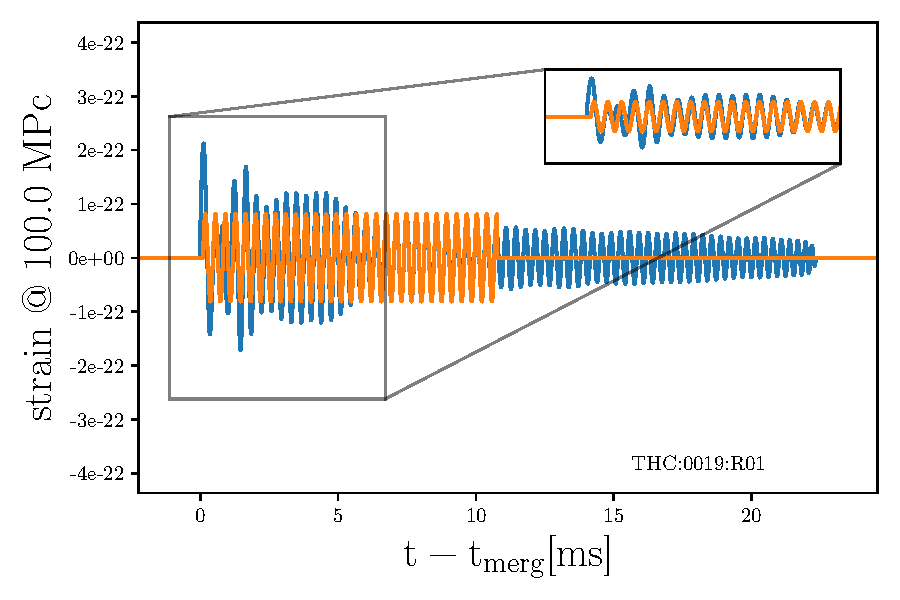
\includegraphics[scale=0.45]{images/Data_analysis/results/2D_grid_12.pdf}
\end{minipage}
\captionsetup{width=0.8\textwidth}
\caption{Spinning BNS waveform and its best monochromatic match}
\caption*{This plot shows the recovered SNR \ref{} for the waveform THC:0019:R01 of the CoRe BNS catalog \cite{}(see figure\ref{} to read the BNS poperties) and the template model \ref{}. The best matching parameters are $f=Hz$, $d=ms$.}
\end{center}
\end{figure}

\FloatBarrier



Since eccentric, high mass ratio, or spinning BNS systems may generate waveforms that are a challenging task for the monochromatic model \ref{}. We can avoid searching in the low frequency region by a different question that slightly modifies the target of the search:

Original question$\rightarrow$" Which parameters f and d would produce the monochromatic wave that recovers most of the signal-to-noise ratio?"

New question$\rightarrow$" Which parameters f and d would produce the monochromatic wave that recovers most of the signal-to-noise ratio that contains more than n oscillations?"


Modifying the question in such a way would increase the number of rejected points lying on the orange region(see figure\ref{fig:11}) and get rid of the loud low-frequency structure dominating the colormaps \ref{} which is related to oscillations right after $t_{merg}$.


\begin{itemize}[leftmargin=*]


\item High mass ratio waveform, using constraint n=15

\begin{figure}[!htbp]
\begin{center}
\begin{minipage}[t]{0.5\linewidth}
\vspace{0pt}
%\raggedleft
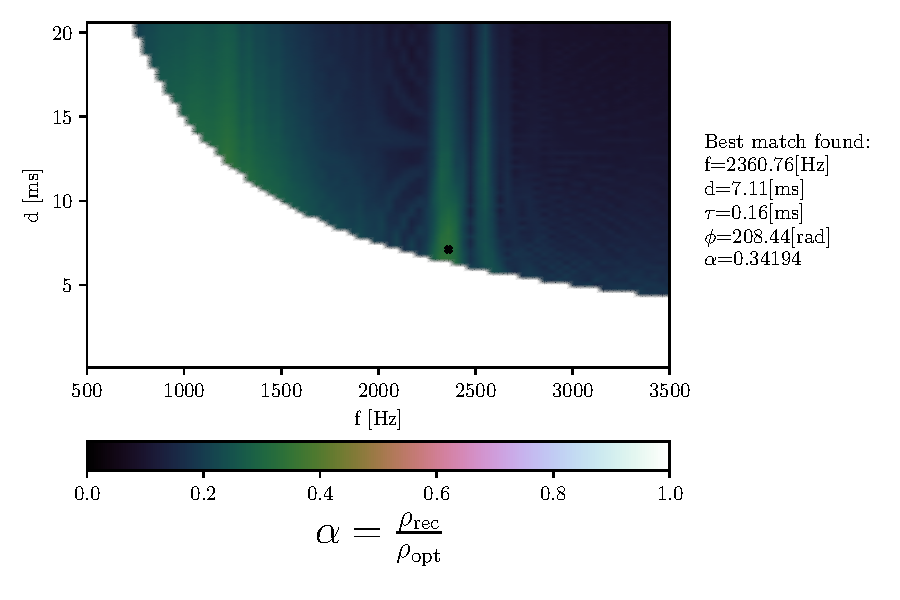
\includegraphics[scale=0.6,trim={2mm 0 35mm 0},clip]{images/Data_analysis/results/2D_grid_13.pdf}
\end{minipage}%
\begin{minipage}[t]{0.5\linewidth}
\vspace{20pt}
%\raggedright
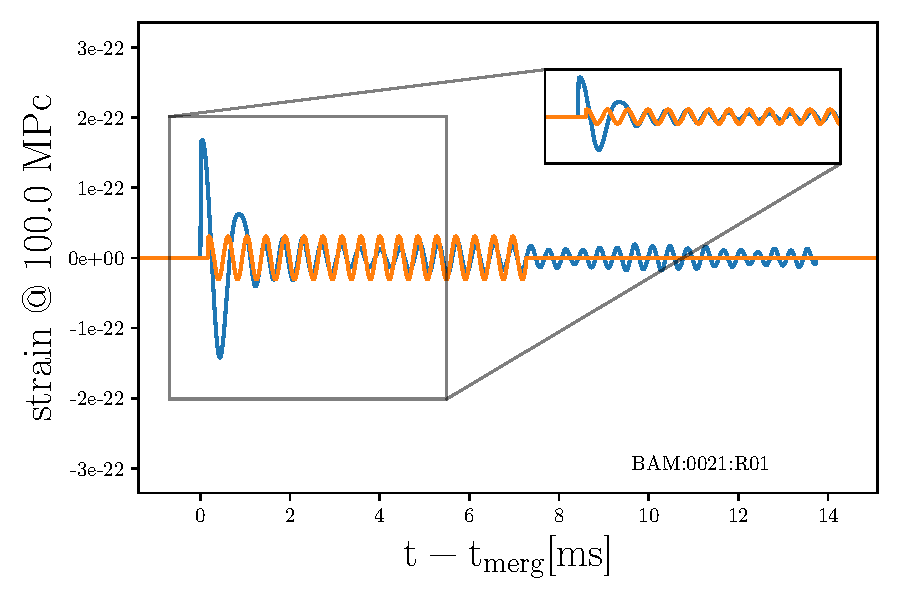
\includegraphics[scale=0.45]{images/Data_analysis/results/2D_grid_14.pdf}
\end{minipage}
\captionsetup{width=0.8\textwidth}
\caption{Spinning BNS waveform and its best monochromatic match}
\caption*{This plot shows the recovered SNR \ref{} for the waveform THC:0019:R01 of the CoRe BNS catalog \cite{}(see figure\ref{} to read the BNS poperties) and the template model \ref{}. The best matching parameters are $f=Hz$, $d=ms$.}
\end{center}
\end{figure}

\FloatBarrier


\item Highly eccentric waveform, using constraint n=15

\begin{figure}[!htbp]
\begin{center}
\begin{minipage}[t]{0.5\linewidth}
\vspace{0pt}
%\raggedleft
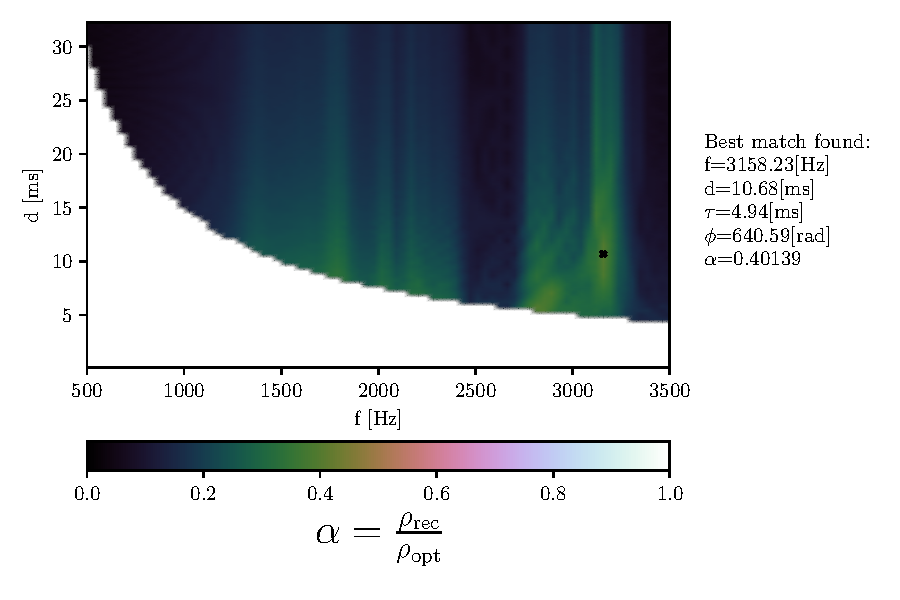
\includegraphics[scale=0.6,trim={2mm 0 35mm 0},clip]{images/Data_analysis/results/2D_grid_15.pdf}
\end{minipage}%
\begin{minipage}[t]{0.5\linewidth}
\vspace{20pt}
%\raggedright
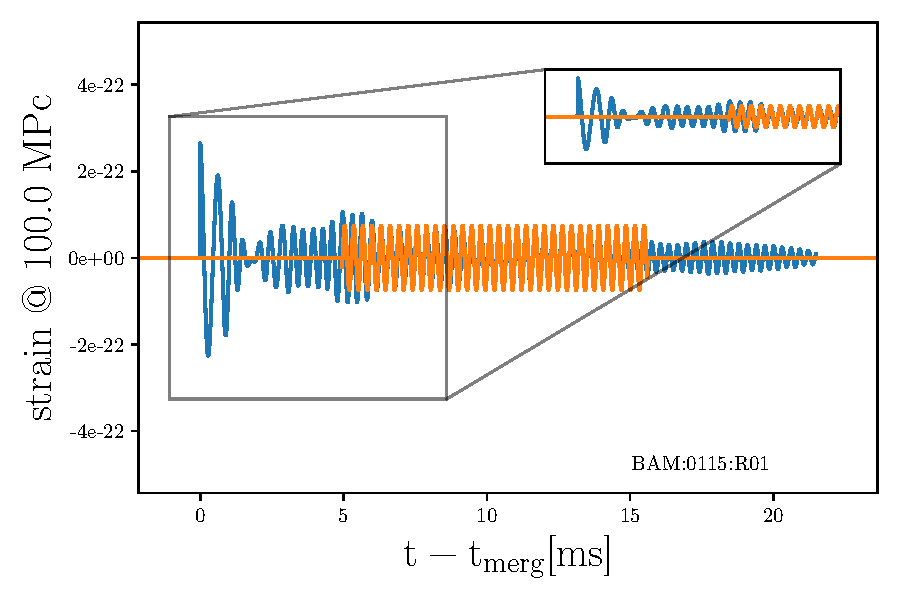
\includegraphics[scale=0.45]{images/Data_analysis/results/2D_grid_16.pdf}
\end{minipage}
\captionsetup{width=0.8\textwidth}
\caption{Spinning BNS waveform and its best monochromatic match}
\caption*{This plot shows the recovered SNR \ref{} for the waveform THC:0019:R01 of the CoRe BNS catalog \cite{}(see figure\ref{} to read the BNS poperties) and the template model \ref{}. The best matching parameters are $f=Hz$, $d=ms$.}
\end{center}
\end{figure}

\FloatBarrier

\end{itemize}


Even though imposing such constraints on parameter space might help recovering the template frequency and duration, using such method in real GW searches seems unfeasible as the start of a GW signal in the datastream is unkonwn and its duration as well.

\newpage
\section{How well can the monochromatic model recover signals in the catalog?}


The fact that a monochromatic template model can recover up to 75\% of the optimal SNR for some waveforms while covering a significant amount of duration like the one shown in figure \ref{BAM:0035} lead us to ask how the model would perform in a more extensive set of waveforms. 


The following section will use a 2-dimensional version of equation \ref{} for a set of j=220 waveforms, to explore possible correlations between signal properties like its main frequency and duration and physical obsevables  using the infrastructure described in figure \ref{}

\begin{equation}\label{eq:21}
\rho_{_{_{rec}}} = \rho^j_{_{_{f,d}}} = \frac{\langle h, q_{_{_{f,d}}}\cdot e^{i(2\pi \tau+\phi)}\rangle \bigg\rvert_{\phi =\phi_{opt},\tau =\tau_{max}}}{\sqrt{\langle  q_{_{_{f,d}}},q_{_{_{f,d}}} \rangle}}
\end{equation}



%The maximum recovered SNR, its location in parameter space $(f,d)$, and the computed amplitude averaged quantities \ref{}, and \ref{} will be computed to do aln analysis containing all waveform types shown in section \ref{2dsearch} would help us figure out whether the "worse" case with poor length recovery shown in figures \ref{BAM:0021} and \ref{BAM:0115} is somewhat more frequent. 

Let $f_{best}$ and $d_{best}$ be the best matching parameters that fit a monochromatic template \ref{} to a postmerger waveform in the catalog \ref{} with amplitude weighted averages $f_{wei}$ and $d_{wei}$ (see equations \ref{},\ref{}). The following ratios will be computed and used to analyze the whole dataset 


\begin{equation}\label{alpha}
\alpha = \frac{\rho_{_{_{rec}}}}{\rho_{opt}}
\end{equation}

\begin{equation}\label{beta}
\beta = \frac{d_{best}}{d_{postm}}
\end{equation}

\begin{equation}\label{betawei}
\beta_{wei} = \frac{d_{best}}{2\cdot d_{wei}}
\end{equation}

\begin{equation}\label{gammawei}
\gamma_{wei} = \frac{f_{best}}{f_{wei}}
\end{equation}

Where $\rho_{opt}$ is the waveform's optimal SNR, and $d_{postm}$ is the cutoff postmerger duration defined in section \ref{}. Several 2D planes will be used to characterize the dataset, keeping fixed the optimal SNR in the y-axis, as we are interested in the detectability of waveforms at 100 MPc. We impose an SNR  threshold of 8, which is picked according to third-generation detector sensitivity, and population studies like \cite[section 3]{https://doi.org/10.48550/arxiv.2109.09882}


\begin{figure}[hbt!]
\begin{center}
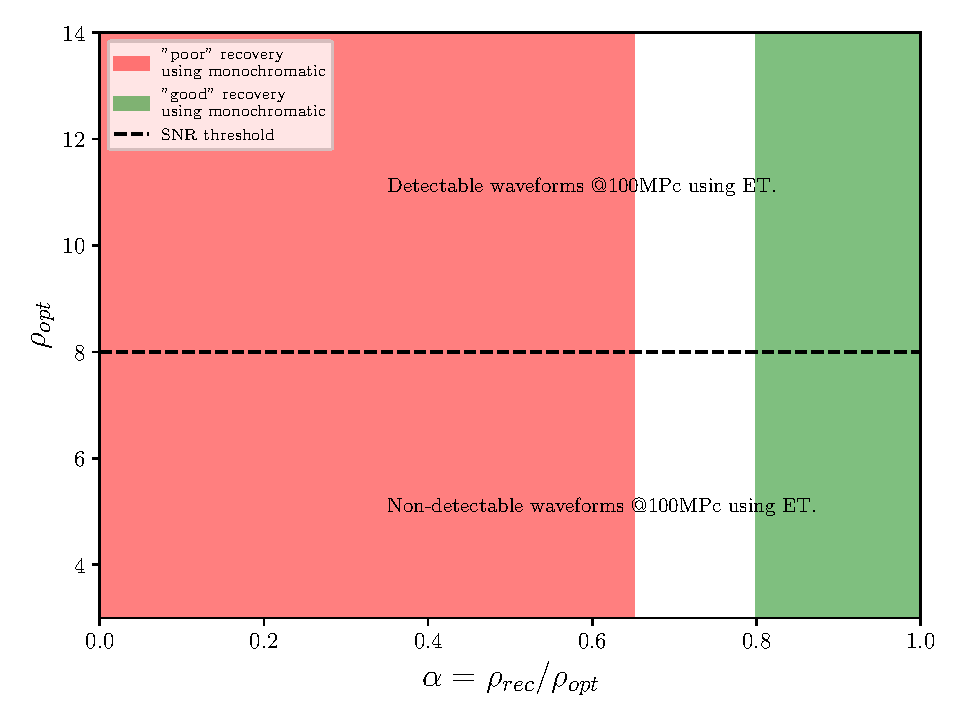
\includegraphics[width=0.5\textwidth, angle=0]{images/Data_analysis/results/schematics.pdf}
\captionsetup{width=0.8\textwidth}
\caption{Detectablity and features of a waveform catalog}
\caption*{This figure depicts the way the dataset will be divided and characterized in terms of optimal SNR \ref{}, and several other "parameters" \ref{alpha}, \ref{beta}, \ref{betawei}, \ref{gammawei}.}
\label{regions}
\end{center} 
\end{figure}

\FloatBarrier

Let us begin by replacing the x-axis of figure \ref{regions} with the SNR recovery \ref{}. The following figure shows side by side the SNR recovery vs the optimal SNR of all waveforms in the dataset. It shows side by side the whole dataset(left) and the waveforms above the optimal SNR threshold(right)


\begin{figure}[hbt!]
\begin{center}
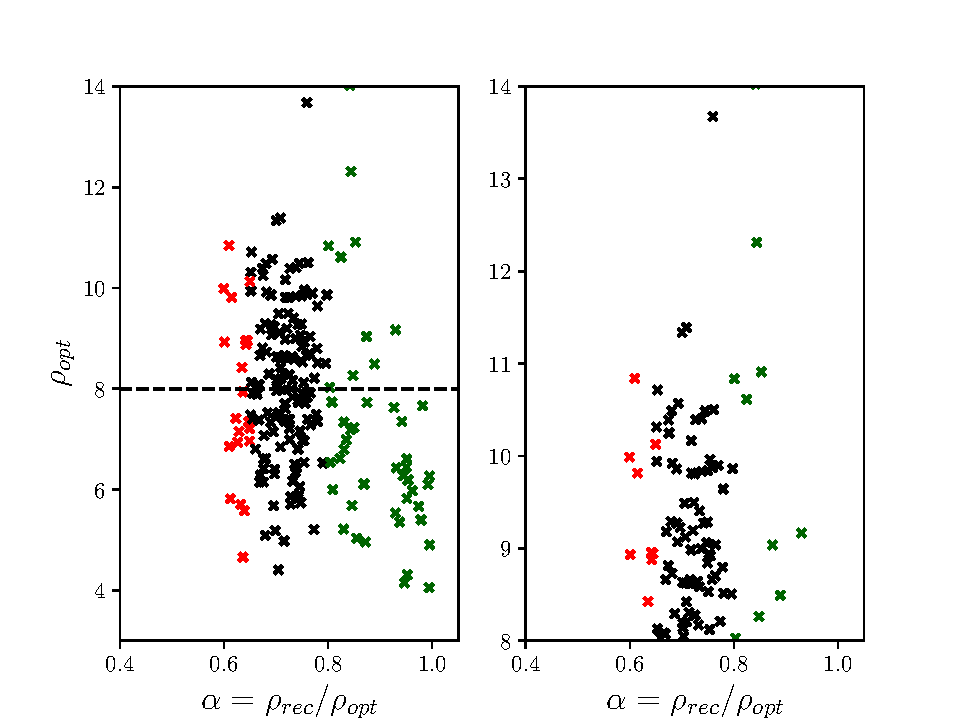
\includegraphics[width=\textwidth, angle=0]{images/Data_analysis/results/alpha_scatter.pdf}
\caption{Signal to noise recovery for the catalog}
\label{ascatter}
\end{center}
\end{figure}

\FloatBarrier


The four corners such figure can be read according to the schematics of figure \ref{} as follows:

\begin{itemize}
\item Upper left: signals that could be detected at 100 MPc, but the monochromatic model leaves a considerable margin of improvement.
\item Lower left: signals that would not be detected at 100 MPc, nor the monochromatic, represents a good model for them.
\item 
Upper right: possibly detectable waveforms at 100MPc that require simple modeling.
\item 
Lower right: non-detectable waveforms at 100MPc that require simple modeling.
\end{itemize}

\newpage

In what follows, histograms will be used to count where   "red" and "green" sample waveforms lie in other dimensions. The same separation will be used to stablish a difference between waveforms above and below the optimal SNR threshold.

First consider histograms for the amplitude weighted frequency and duration

\begin{figure}[hbt!]
\begin{center}
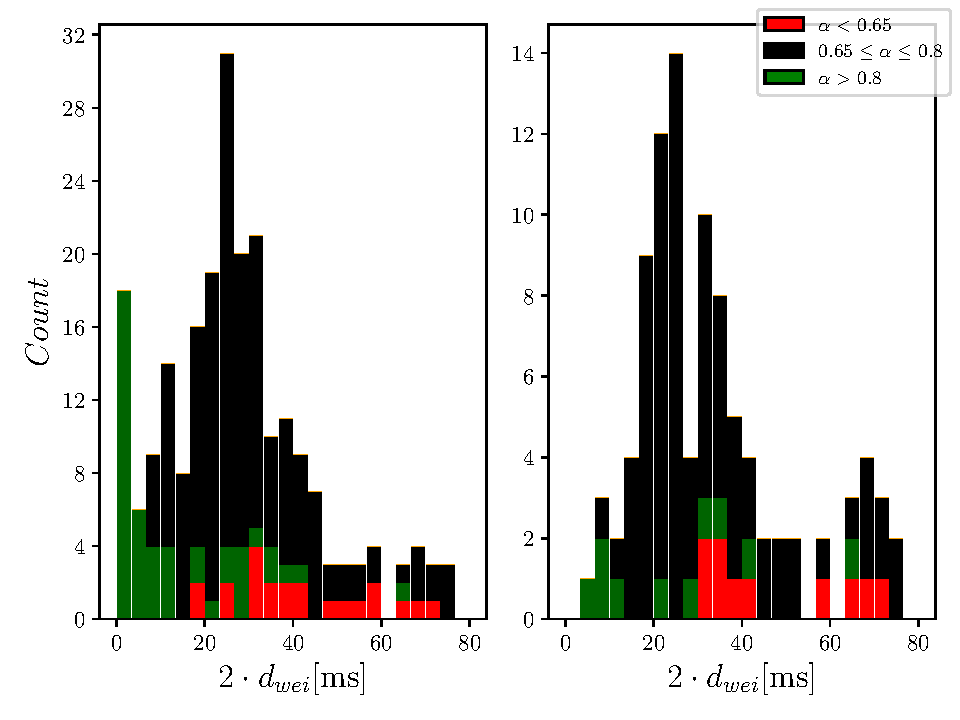
\includegraphics[width=0.8\textwidth, angle=0]{images/Data_analysis/results/alpha_dhist.pdf}
\caption{Amplitude weighted durations in the catalogs}
\label{adhist}
\end{center}
%This figure shows two histograms for the amplitude weighted duration $2\cdot d_{wei}$; It follows the recovery color scheme of figure \ref{regions}. The one on the left accounts for the whole set of waveforms and the one on the right, only the ones lying above the threshold.
\end{figure}

\begin{figure}[hbt!]
\begin{center}
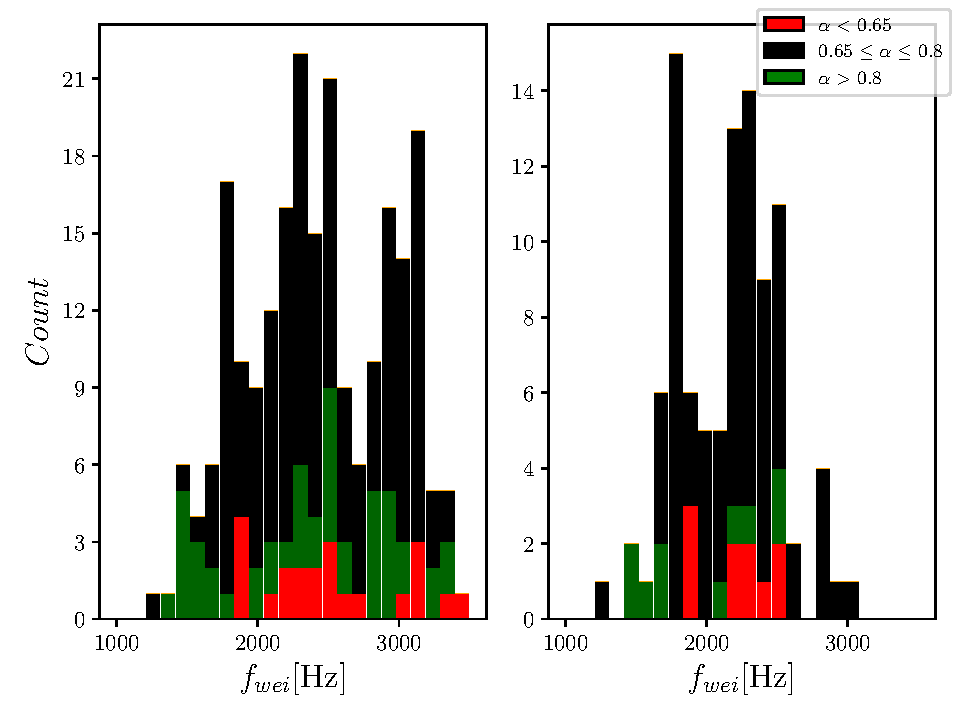
\includegraphics[width=0.8\textwidth, angle=0]{images/Data_analysis/results/alpha_fhist.pdf}
\caption{Amplitude weighted frequencies in the catalogs}
\label{afhist}
\end{center}
%This figure shows two histograms for the amplitude weighted frequency $f_{wei}$; It follows the recovery color scheme of figure \ref{regions}. The one on the left accounts for the whole set of waveforms and the one on the right, only the ones lying above the threshold.
\end{figure}
\FloatBarrier


Notice how transitioning from the whole dataset(left) to only above threshold waveforms(right) does two different things: It significantly reduces the tall green bar in figure \ref{}  and its neighboring bars. In addition, in figure \ref{} we see how most green bars disappear around the 3000Hz value in the weighted frequency histogram. Combining both plots we can tell that the lower green region in figure \ref{} contains many short waveforms with high average frequency.

Moreover, the red samples tell us how the monochromatic template model struggles to get more than 65\% of the optimal SNR for waveforms longer than 30 milliseconds. 


\newpage 

With regards to the parameters found for the monochromatic match on each waveform of the catalog, we can use the histograms for the quantities  $\beta$ and $\gamma_{wei}$ 

\begin{figure}[hbt!]
\begin{center}
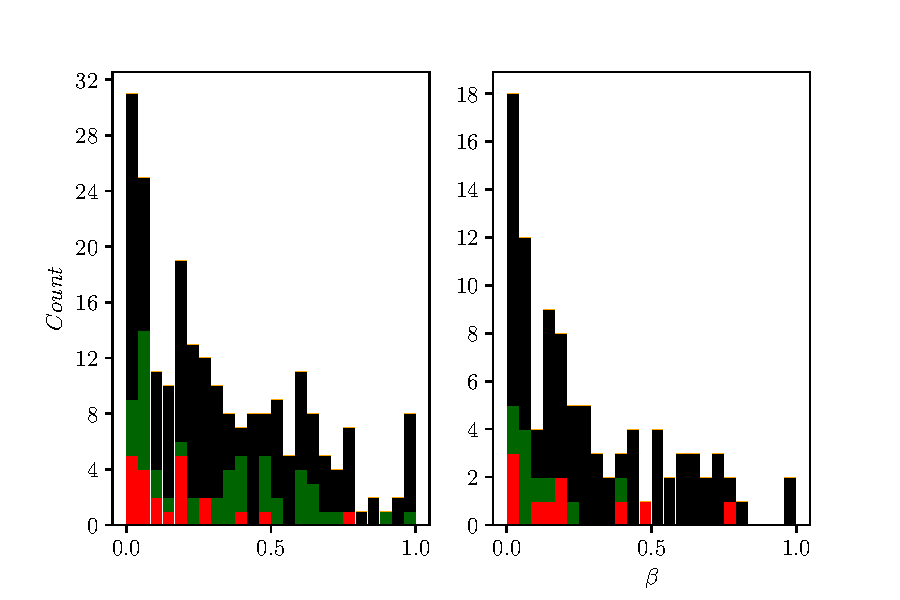
\includegraphics[width=0.8\textwidth, angle=0]{images/Data_analysis/results/alpha_betahist.pdf}
\caption{Duration recovery in the catalogs}
\label{abhist}
\end{center}
%This figure shows two histograms for the ratio of durations  $\beta$ defined in equation \ref{beta}; It follows the recovery color scheme of figure \ref{regions}. The one on the left accounts for the whole set of waveforms and the one on the right, only the ones lying above the threshold.
\end{figure}

\begin{figure}[hbt!]
\begin{center}
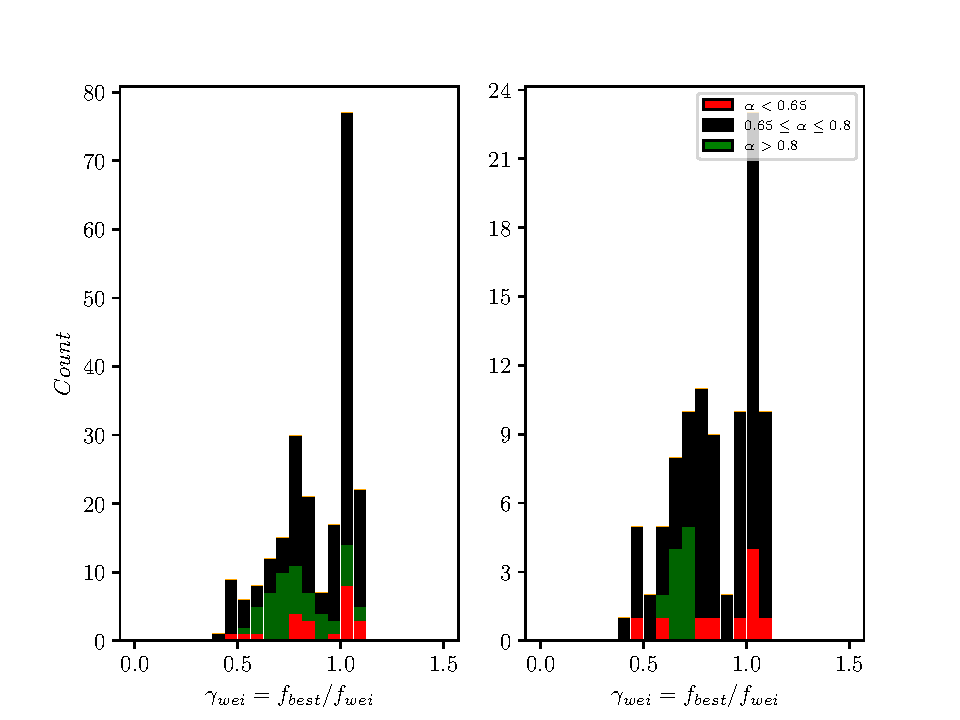
\includegraphics[width=0.8\textwidth, angle=0]{images/Data_analysis/results/alpha_gammahist.pdf}
\caption{Frequency recovery in the catalogs}
\label{aghist}
\end{center}
%This figure shows two histograms for the ratio of durations  $\gamma_{wei}$ defined in equation \ref{gammawei}; It follows the recovery color scheme of figure \ref{regions}. The one on the left accounts for the whole set of waveforms and the one on the right, only the ones lying above the threshold.
\end{figure}
\FloatBarrier

Where the closer to 1.0, the better recovery of the signal duration and frequency one gets. Some waveforms in the green region recover the duration and weighted frequency well, but many green bars disappear as we go above the threshold. As previously seen, the red bars mainly belong to long waveforms, for which, the monochromatic template performs very poorly recovering its length, regardless of whether the right weighted frequency was properly recovered, as the red bars seem very spread out in the $\gamma_{wei}$ histogram. 

\newpage

Let us now, take a look at physical observables like the system's total mass, mass ratio, and effective spin $\chi_{eff}$.  

\begin{figure}[hbt!]
\begin{center}
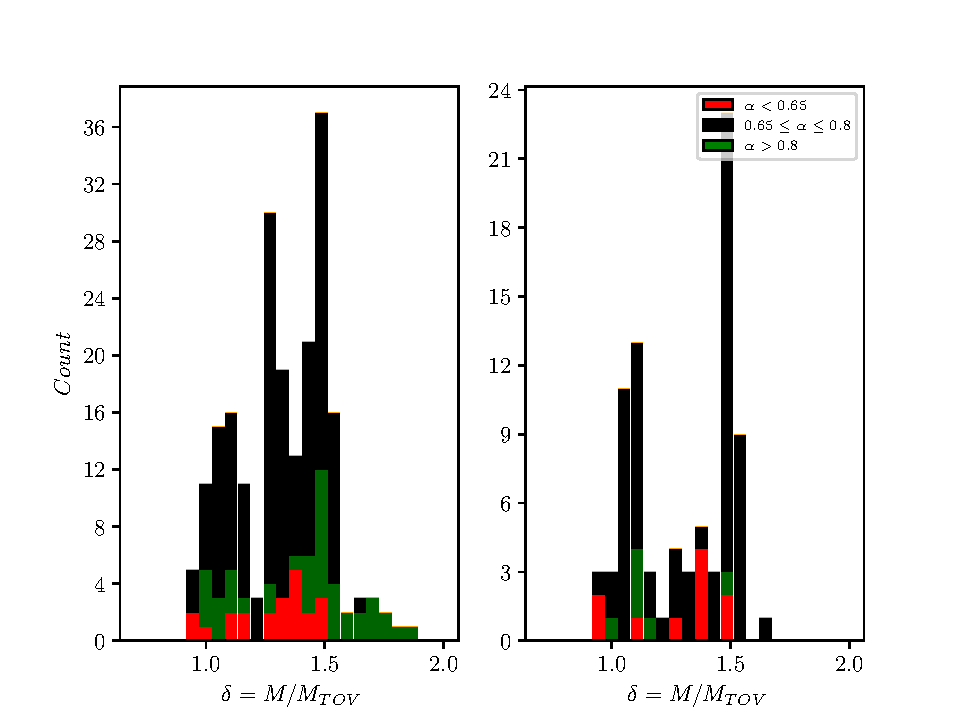
\includegraphics[width=0.8\textwidth, angle=0]{images/Data_analysis/results/alpha_deltahist.pdf}
\caption{Total mass of the systems in the catalogs}
\label{adelhist}
\end{center}
%This figure shows two histograms for the physical obsevable $\delta$ defined in equation \ref{delta}; It follows the recovery color scheme of figure \ref{regions}. The one on the left accounts for the whole set of waveforms and the one on the right, only the ones lying above the threshold.
\end{figure}

Counting the waveforms lying in the region where $\delta>1.6$ one can see that the green bars present in the whole dataset(left) dissapear in the above threshold dataset(right). Such set of signals can be identified as short high-frequency signals that belong to heavy systems. 

\begin{figure}[hbt!]
\begin{center}
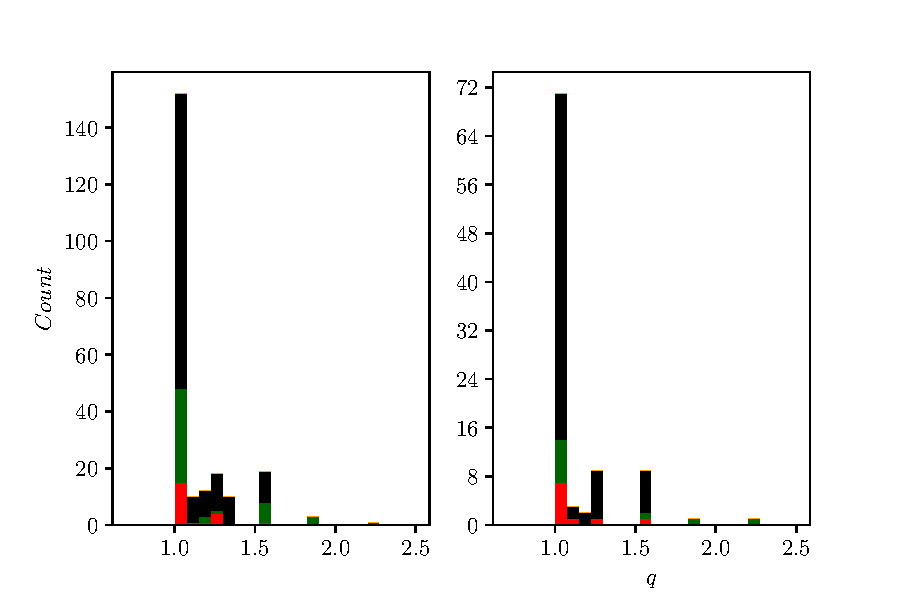
\includegraphics[width=0.8\textwidth, angle=0]{images/Data_analysis/results/alpha_qhist.pdf}
\caption{Mass ratio of the systems in the catalogs}
\label{aqhist}
\end{center}
%This figure shows two histograms for the mass ratio $q$; It follows the recovery color scheme of figure \ref{regions}. The one on the left accounts for the whole set of waveforms and the one on the right, only the ones lying above the threshold.
\end{figure}

The waveform dataset is dominated by equal mass waveforms, so by looking at the few waveform samples with  high mass ratio $q=m_1/m_2>1.6$, one can see that the green bars survive the threshold cut, which means they lie in the upper right region of plot \ref{}, making them good candidates for detection.
 

\newpage

Finally spinning BNS systems, i.e. $\chi_{eff}>0.2$ are also a small subset in this catalogs, as many waveforms come from non-spinning systems. Nevertheless, one can also see that the green bars survive the threshold cut, which means they lie in the upper right region of plot \ref{}, making them good candidates for detection..

\begin{figure}[hbt!]
\begin{center}
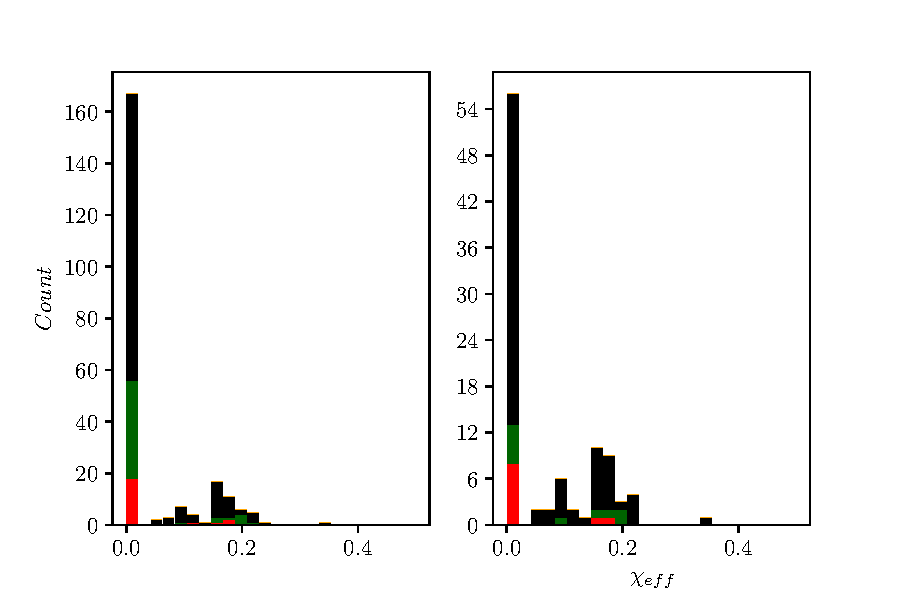
\includegraphics[width=0.8\textwidth, angle=0]{images/Data_analysis/results/alpha_chihist.pdf}
\caption{Spining systems in the catalogs}
\label{achihist}
\end{center}
This figure shows two histograms for the effective spin parameter $\chi_eff$ defined in equation \ref{chieff}; It follows the recovery color scheme of figure \ref{regions}. The one on the left accounts for the whole set of waveforms and the one on the right, only the ones lying above the threshold.
\end{figure}

\FloatBarrier

\subsection*{Findings}

Overall the monochromatic template model performance over the whole catalog shows that it is possible to recover between 65-98\% of the optimal signal-noise ratio. However, most of the best candidates(above 90\% of recovery) are short and high-frequency postmerger phases that would not be detectable at 100MPc if a threshold SNR of 8 is imposed. On the other hand, high mass ratio and eccentric binaries are detectable and have a very good SNR recovery due to loud oscillations after the maximum amplitude of the l=2,m=2 mode. However, better amplitude or phase modeling would be required as there is a poor duration recovery.

Overall the monochromatic template model seems to perform decently when it comes to equal mass non-precessing waveforms, having an SNR recovery between 65-85\% of the optimal, where in most cases, a good portion of its length and weighted frequency are correctly recovered.

\begin{figure}[hbt!]
\begin{center}
\begin{tabular}{cc}
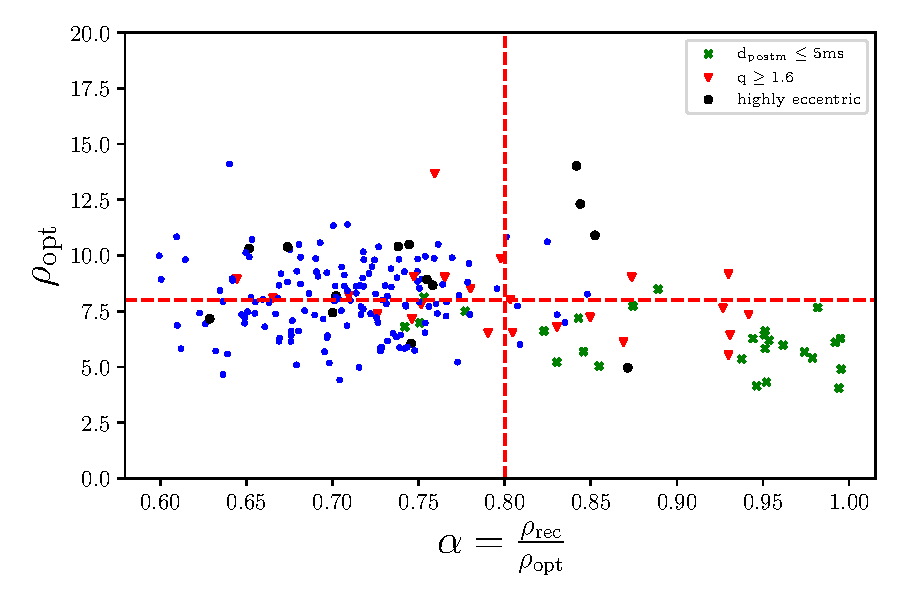
\includegraphics[width=0.7\textwidth, angle=0]{images/Data_analysis/results/alpha_sum0.pdf}
\end{tabular}
\end{center}
\caption{$\alpha - \rho_{opt}$ and $\beta - \alpha$  planes}
This figure summarizes the search findings over the BNS waveform database according to \ref{regions}. The plot on the left uses different markers and colors to show the best waveform candidates, and the plot on the right the weaknesses of the monochromatic template model \ref{eq:20}.
\end{figure}

\begin{figure}[hbt!]
\begin{center}
\begin{tabular}{cc}
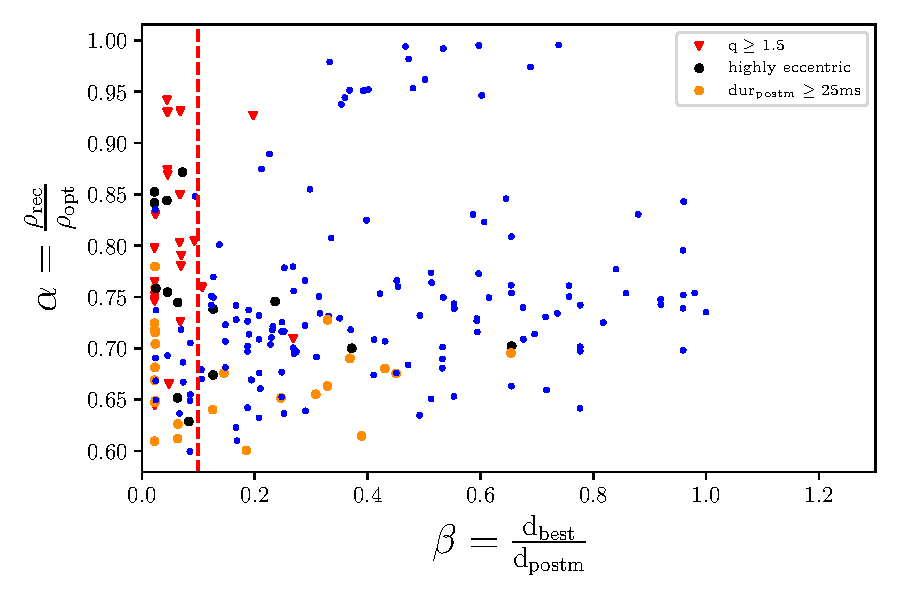
\includegraphics[width=0.7\textwidth, angle=0]{images/Data_analysis/results/alpha_sum1.pdf}
\end{tabular}
\end{center}
\caption{$\alpha - \rho_{opt}$ and $\beta - \alpha$  planes}
This figure summarizes the search findings over the BNS waveform database according to \ref{regions}. The plot on the left uses different markers and colors to show the best waveform candidates, and the plot on the right the weaknesses of the monochromatic template model \ref{eq:20}.
\end{figure}
\FloatBarrier


\newpage
\section{Monochromatic models with modified amplitude envelopes}\label{zc-aenv}
One of the most characteristic features of a postmerger BNS signal is the first amplitude minimum after the merger, as seen in figure \ref{fig:9}, which appears in every waveform of the catalog. A first attempt to improve the template model could be modifying the constant amplitude of the monochromatic model with a zero-crossing amplitude envelope. 

A wide variety of known functions could model such a feature; nevertheless, this analysis will focus on: a piecewise linear function with zero crossing and a hyperbolic tangent function. Further, one could propose models that, instead of crossing the zero line, touch it tangentially and return symmetrically to its original state. The absolute value of the piecewise linear model and a squared hyperbolic tangent model would reproduce such behavior.

\vspace{1cm}

\begin{itemize}
\item zero-crossing:
\begin{equation}\label{line}
Y0_{w, t_{min}}(t) =
\begin{cases} 
      1 &, t<t_{min}-\mathrm{\frac{width}{2}} \\
      \left( \frac{-2A}{\mathrm{width}} \right) \cdot (t- t_{min}) &, t_{min}-\mathrm{\frac{width}{2}} \leq t \leq t_{min}+\mathrm{\frac{width}{2}} \\
     -1 &, t>t_{0}+d
   \end{cases}
\end{equation}

\begin{equation}\label{tanh}
Y1_{\epsilon, t_{min}}(t) = A \cdot \tanh (\epsilon \cdot(t-t_{min}))
\end{equation}

\vspace{0.5cm}


\item zero-touching:
\begin{equation}\label{line-abs}
Y2_{w, t_{min}}(t) = \left| Y0_{w, t_{min}}(t) \right|
\end{equation}

\begin{equation}\label{tanh2}
Y3_{\epsilon, t_{min}}(t) = \left( Y0_{\epsilon, t_{min}}(t) \right)^2
\end{equation}

\end{itemize}

Then the new templated model acquires 2-more parameters, one that controls where the zero-crossing happens and the other the width of the region where the envelope has this behavior.

\begin{equation}\label{4dim-model}
U0_{_{f,d, w, tmin}} = Y0_{_{w,t_{min}}}(t) \cdot
\begin{cases} 
      0 & t<t_{0_{opt}} \\
      A_{opt} \cdot sin(2\pi f t + \phi_{0_{opt}}) & t_{0_{opt}} \leq t\leq t_{0_{opt}}+d \\
      0 & t>t_{0_{opt}}+d
   \end{cases}
\end{equation}


Even though template models of the form \ref{4dim-model} seem would translate the problem into a 4-dimensional search, one could keep the dimensionality low by using universal relations like [ref dietrich], which tell the location of the first minimum with respect to maximum amplitude. 

Finally, the template model can be posed as a 2D+1 when fixing the $t_{min}$ but leaving the width as a free parameter.

\begin{equation}\label{3dim-model}
U0_{_{f,d, w}} = Y0_{_{w}}(t) \cdot
\begin{cases} 
      0 & t<t_{0_{opt}} \\
      A_{opt} \cdot sin(2\pi f t + \phi_{0_{opt}}) & t_{0_{opt}} \leq t\leq t_{0_{opt}}+d \\
      0 & t>t_{0_{opt}}+d
   \end{cases}
\end{equation}

\begin{figure}[hbt!]
\begin{center}
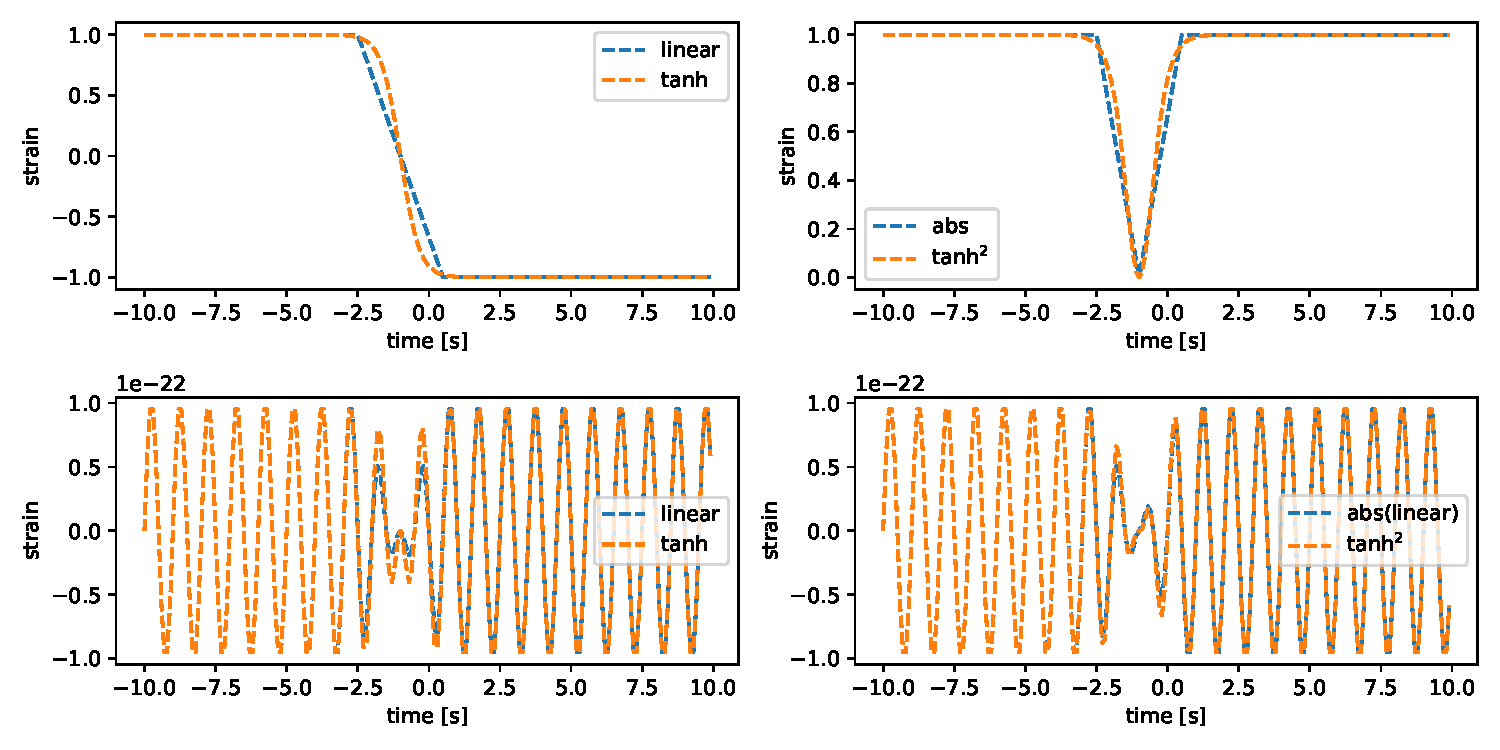
\includegraphics[width=\textwidth, angle=0]{images/Data_analysis/results/envel.pdf}
\caption{modified envelopes on monochromatic waves}
\label{env.ex}
\end{center}
Envelopes \ref{tanh2}, \ref{tanh}, \ref{line} acting on a monochormatic wave with parameters f=1Hz, d=20s, $t_{0}=-10s$ with a zero crossing at -1s.
\end{figure}
\FloatBarrier

Finding global maxima along slices will give us all the model information; therefore, picturing such parameter space as a stack of the 2D plane will be very useful.

\begin{figure}[hbt!]
\begin{center}
\includegraphics[width=0.5\textwidth, angle=0]{images/3d.png}
\caption{3-dimensional parameter space}
\end{center}
\end{figure}
\FloatBarrier

As seen in previous sections, equal mass and some precessing equal mass waveforms roughly show a simple oscillatory behavior with one deep amplitude minimum. For that reason, we will use models \ref{line}, \ref{line-abs}, and \ref{tanh} and compare results with the ones from the monochromatic model with a constant envelope. Precessing waveforms where the second amplitude minimum has a depth comparable to the first would require a better model.

\newpage

\subsection*{Findings}



\subsubsection*{Non-precessing Equal mass systems}
The search is performed in an 80x80x20 cubic mesh, where the frequency ranges between 2000-2500Hz, and the duration from 5ms to $1.5\cdot d_{postm}$ (see figure \ref{postm_cut}). The width ranges between 1 and 10 ms.




\begin{figure}[hbt!]
\begin{center}
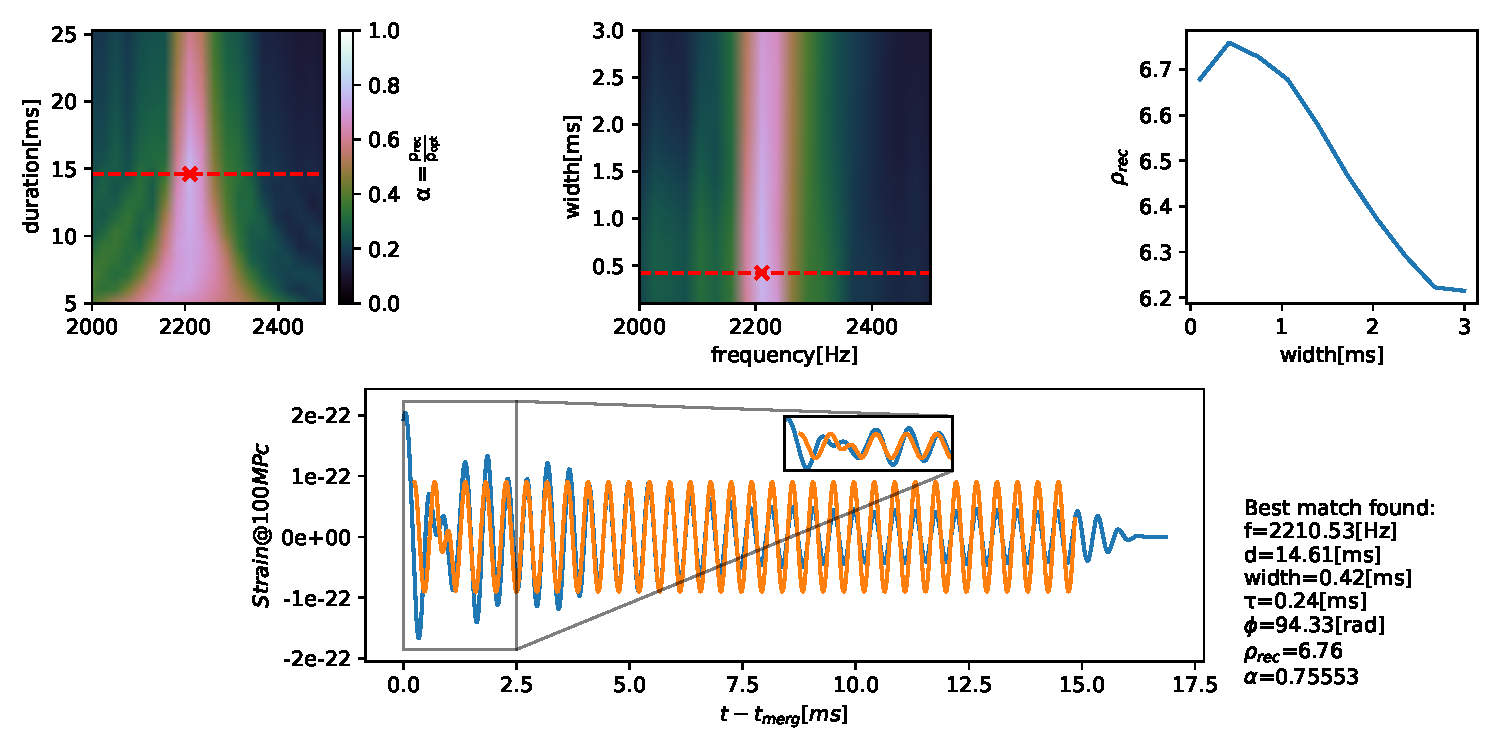
\includegraphics[width=0.6\textwidth, angle=0]{images/Data_analysis/results/envel_35_lin.pdf}
\caption{piecewise linear envelope model}
\end{center}
The search using the piecewise linear envelope model shows an SNR recovery and length marginally different from the one obtained with the monochromatic with constant amplitude model. The minimum amplitude width recovered seems to reproduce well wave shape around the minimum, but the algorithm gets more SNR when matching the tail instead of the first oscillations. 
\end{figure}

\begin{figure}[hbt!]
\begin{center}
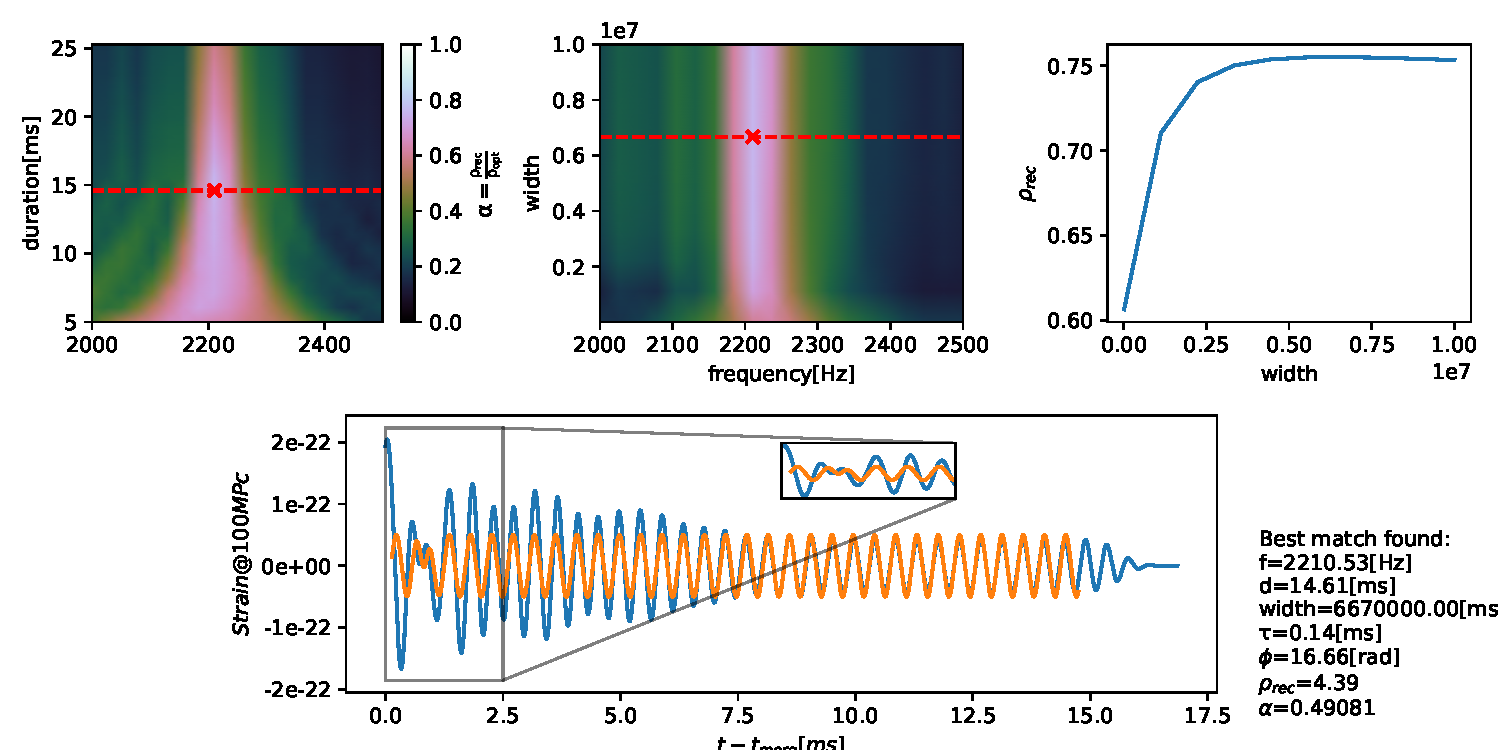
\includegraphics[width=0.6\textwidth, angle=0]{images/Data_analysis/results/envel_35_tanh.pdf}
\caption{$\tanh$ model}
\end{center}
The search using the hyperbolic tangent model shows a worse SNR recovery than the piecewise linear and constant amplitude(monochromatic), even though in the time domain, it seems to match the waveform shape around the amplitude minimum. 
\end{figure}

\begin{figure}[hbt!]
\begin{center}
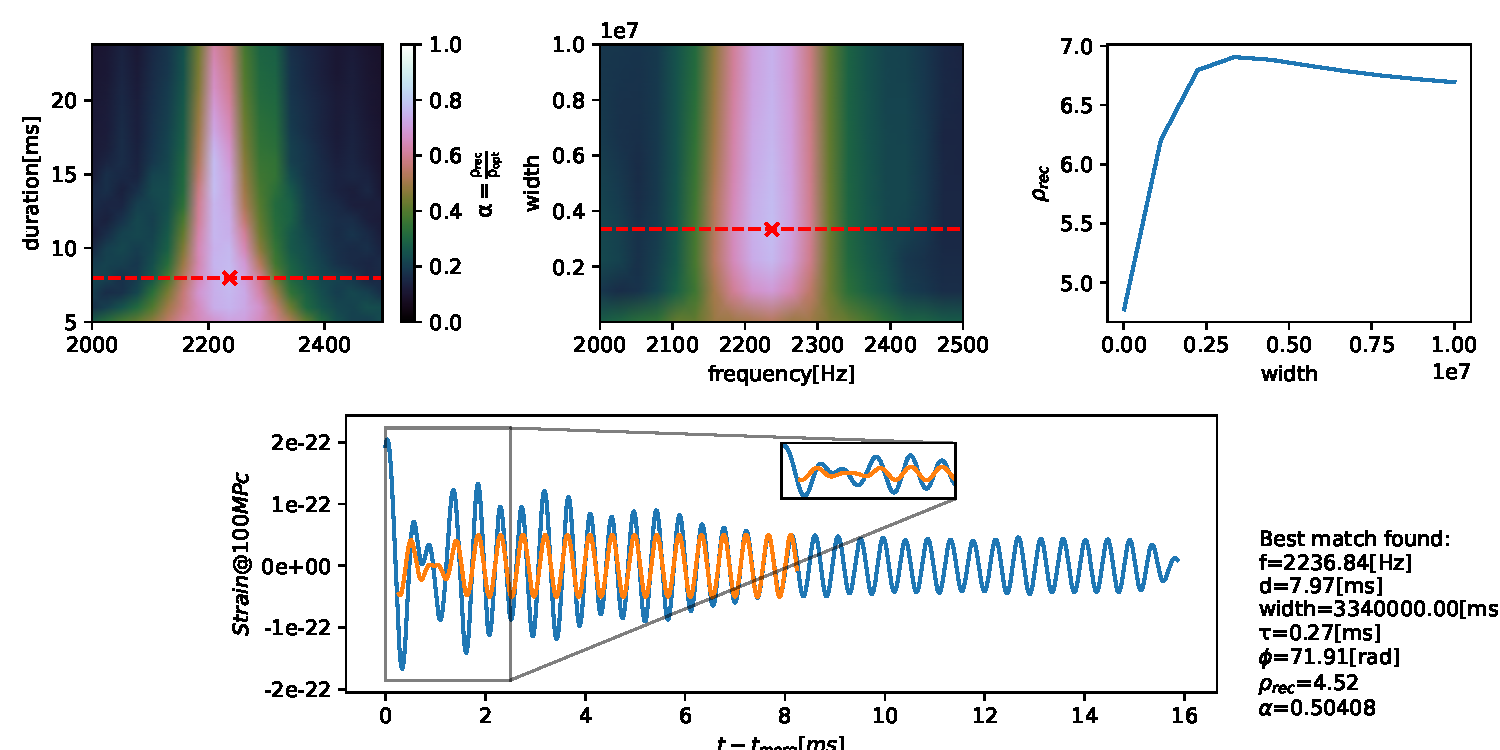
\includegraphics[width=0.6\textwidth, angle=0]{images/Data_analysis/results/envel_35_tanh2.pdf}
\caption{$\tanh^2$ model}
\end{center}
The search using the squared hyperbolic tangent envelope model gives a similar result: worse SNR recovery than the piecewise linear and monochromatic with constant amplitude. However, the length recovery is good, and the shape around the minimum seems to match quite smoothly.
\end{figure}

\FloatBarrier


\subsubsection*{Precessing equal mass waveforms}

Precessing systems may have two types of waveforms, some with one dominant deep amplitude minimum and much small amplitude local modulations. However, also, there are cases where there is a second amplitude minimum of the order of the first one. A better model must be built for the second case, as this analysis considers the first one.

\begin{figure}[hbt!]
\begin{center}
\begin{tabular}{cc}
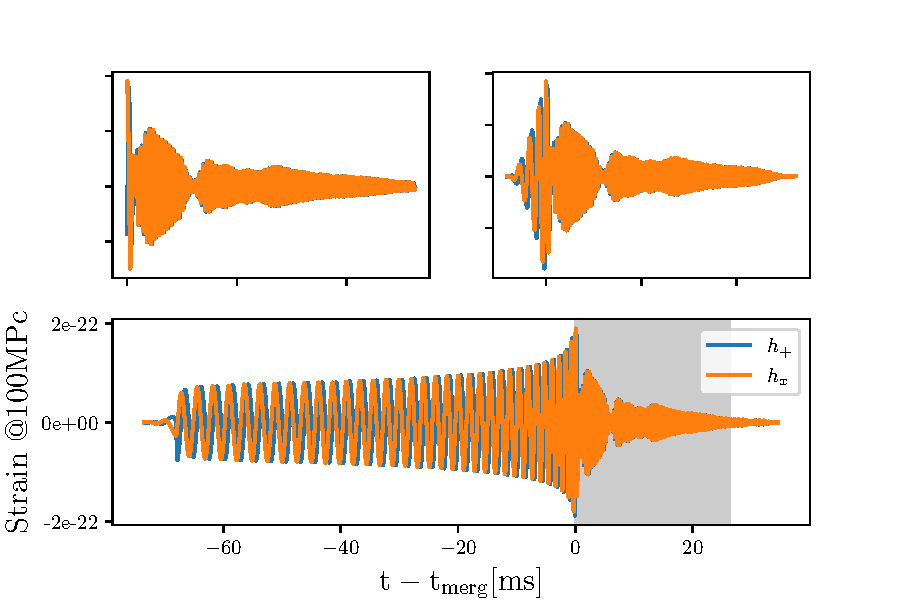
\includegraphics[width=0.45\textwidth, angle=0]{images/Data_analysis/results/d_postm_chi.pdf}

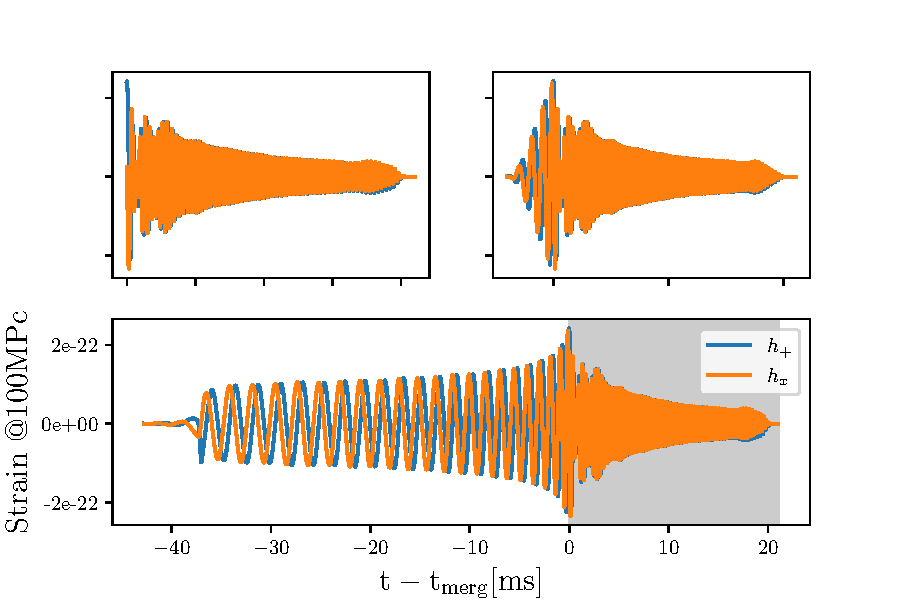
\includegraphics[width=0.45\textwidth, angle=0]{images/Data_analysis/results/d_postm_chi1.pdf}
\end{tabular}
\end{center}
\caption{Precessing waveforms}
This figure shows the two types of precessing waveforms present in the catalog. Many have two deep amplitude minima after the merger(left), but some only have one (right).
\end{figure}

\FloatBarrier





The search is also performed in an 80x80x20 cubic mesh, but the bounds are around the peak of figure \ref{BAM:0106}. The frequency ranges between 3000-3500Hz and the duration from 5ms to $1.5\cdot d_{postm}$(see figure \ref{postm_cut}). The width ranges between 1 and 10 ms.

\begin{figure}[hbt!]
\begin{center}
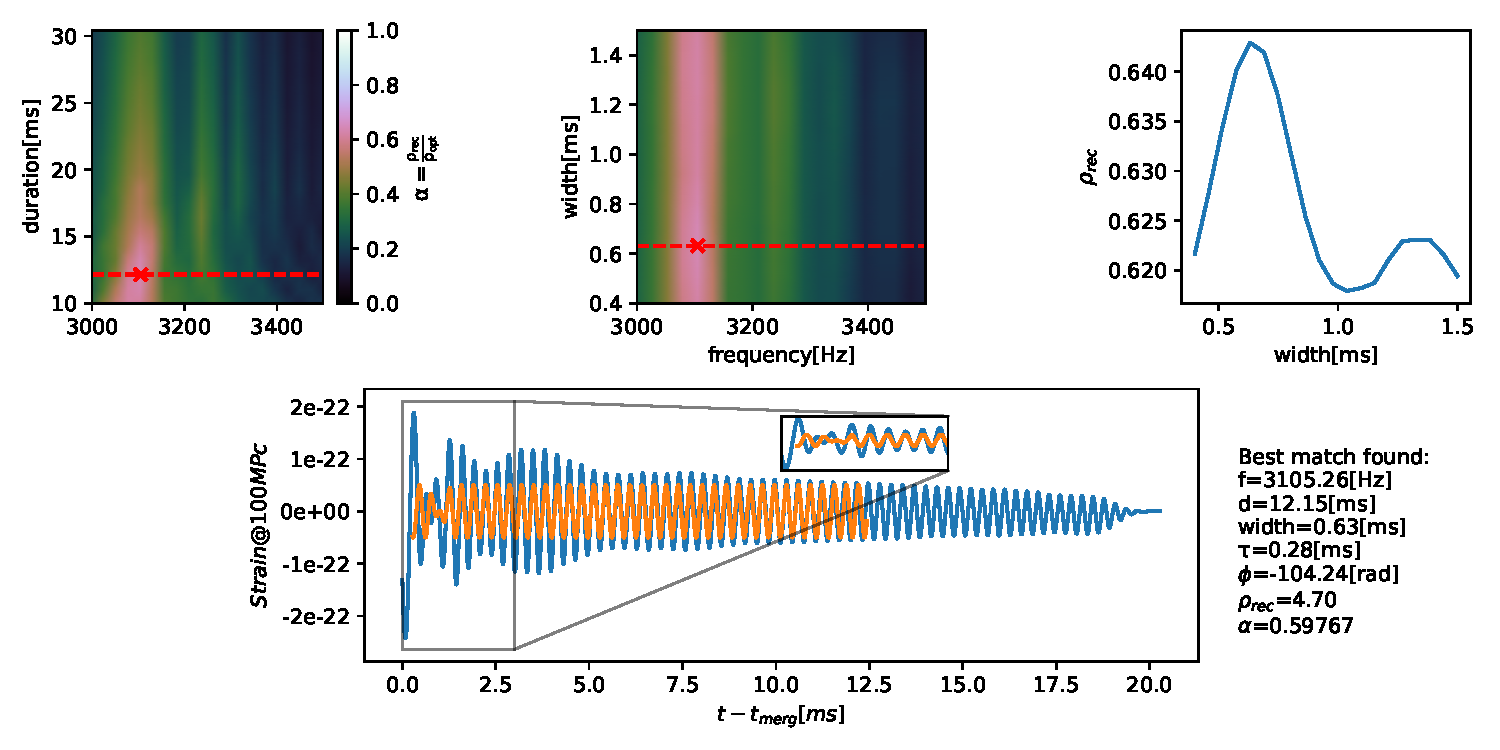
\includegraphics[width=0.6\textwidth, angle=0]{images/Data_analysis/results/envel_110_lin.pdf}
\caption{piecewise linear model for precessing waveforms}
\end{center}
The piecewise linear model reproduces the wave's shape worse around the minimum in the time domain. There is also worse SNR recovery(60\%), but length recovery stays very similar.
\end{figure}

\begin{figure}[hbt!]
\begin{center}
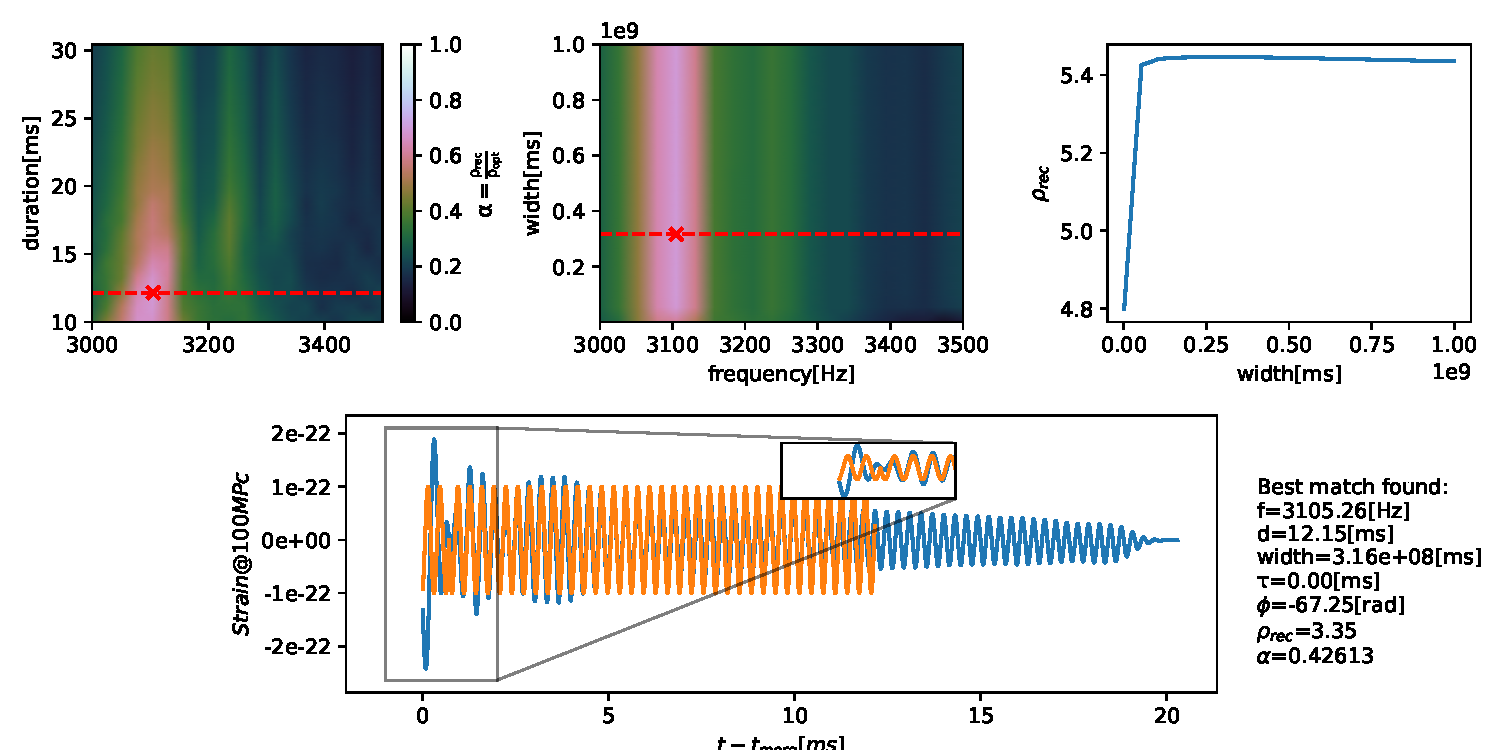
\includegraphics[width=0.6\textwidth, angle=0]{images/Data_analysis/results/envel_110_tanh.pdf}
\caption{$\tanh$ model for precessing systems}
\end{center}
The hyperbolic tangent model struggles to correctly match the first few oscillations but prefers matching the oscillations after the minimum. SNR performs worse(42\%), and length recovery seems unaffected.
\end{figure}

\begin{figure}[hbt!]
\begin{center}
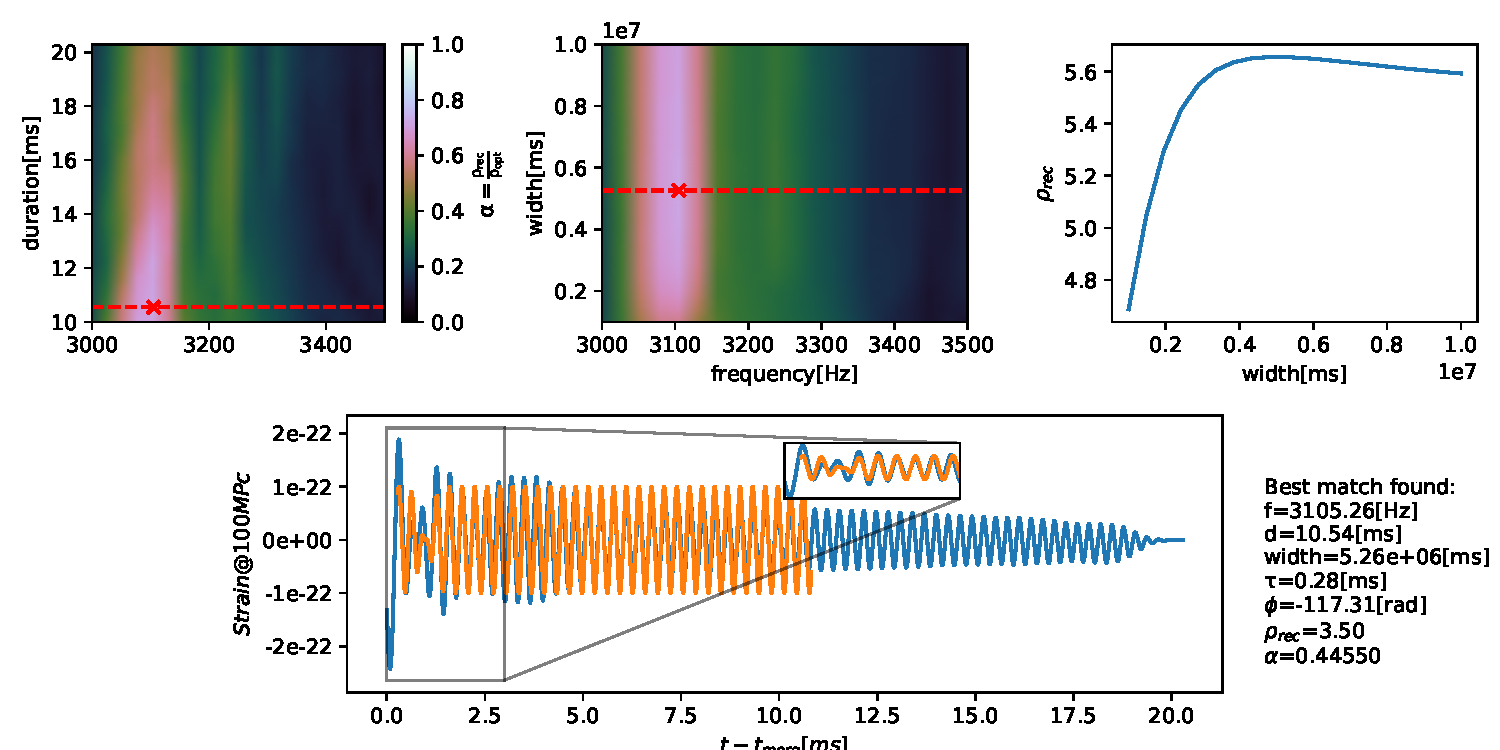
\includegraphics[width=0.6\textwidth, angle=0]{images/Data_analysis/results/envel_110_tanh2.pdf}
\caption{$\tanh^2$ model for precessing systems}
\end{center}
This model seems to match the shape around the minimum in the time domain much better and performs better than the previous one, i.e., it recovers more of SNR(44\%) while the length is also reduced.
\end{figure}

\FloatBarrier

\newpage

Evidence shows that such a model would help recover a similar shape in the time domain around the minimum. However, even in cases where monochromatic with constant amplitude performed the best, i.e., SNR recovery(75\%) and length recovery up to 80\%, non of the models proposed in this section would improve a real search where the signal is not clean. Most likely, the features around the amplitude minimum could not be resolved.

Other types of waveforms, like the ones from heavy systems, with high mass ratio and eccentric, show different morphologies and would need a different amplitude evolution model as they possess different features.



\section{Impacts of amplitude and phase evolution on different postmerger  waveforms}

In general, expecting a simple monochromatic model to match the postmerger phase of any BNS waveform type sounds optimistic. Taking an existing model and adding extra features without considerably increasing its parameter space dimensionality is a very challenging task. Even simple cases like the one proposed in the previous section show that there are cases where(in the time domain)a signal seems to reproduce very well a new feature. In contrast, when used in search pipelines, the new model did not improve or even get worse results. 

Having such a complex morphology on a signal leads us to ask whether the SNR losses come from either part of the amplitude that is not quite well modeled or the misalignments caused by a poorly modeled phase evolution. With so many types of waveforms, one should not expect a single global answer that inclines towards one or the other option.

This analysis will take the phase and amplitude evolution separately, modify simple sinusoidal waves, and test which one gets the closest to a perfect model; the waveform itself.

Building both models could be done by modifying the phase of a sin wave and its amplitude separately. However, to avoid looking for better models of the postmerger amplitude and phase in state-of-the-art literature, this analysis takes the phase and amplitude of the waveform itself. Then, it uses them separately to modify a simple sinusoidal model.

\begin{itemize}

\item Amplitude


\begin{equation}\label{a-evol}
f(t) = |H(t)| \cdot \begin{cases} 
      0 &, t< t_{merg} \\
      sin(2\pi f_{_{best}}\cdot t + \phi_{opt}) &, t_{merg} \leq t \leq t_{merg} + d_{postm} \\
      0 &, t> t_{merg} + d_{postm}
   \end{cases}
\end{equation}

\item Phase

\begin{equation}\label{pha-evol}
g(t) = \cdot \begin{cases} 
      0 &, t< t_{merg} \\
      A \cdot sin(\phi(t)) &, t_{merg} \leq t \leq t_{merg} + d_{postm} \\
      0 &, t> t_{merg} + d_{postm}
   \end{cases}
\end{equation}

\end{itemize}

To avoid the model with amplitude evolution \ref{a-evol} losing a lot of SNR due to misalignments, we first make an intermediate step to find the best frequency and phase of a constant amplitude sin while fixing the length to the length of the waveform. That represents a computationally inexpensive task as it can be formulated as a one-dimensional search.


One may explore all types of waveforms shown in figure \ref{fig:10} by examining what their SNR curves as a timeshift function look like and pay special attention to how close the peaks of each curve compare to the waveform itself.

\begin{figure}[hbt!]
\begin{center}
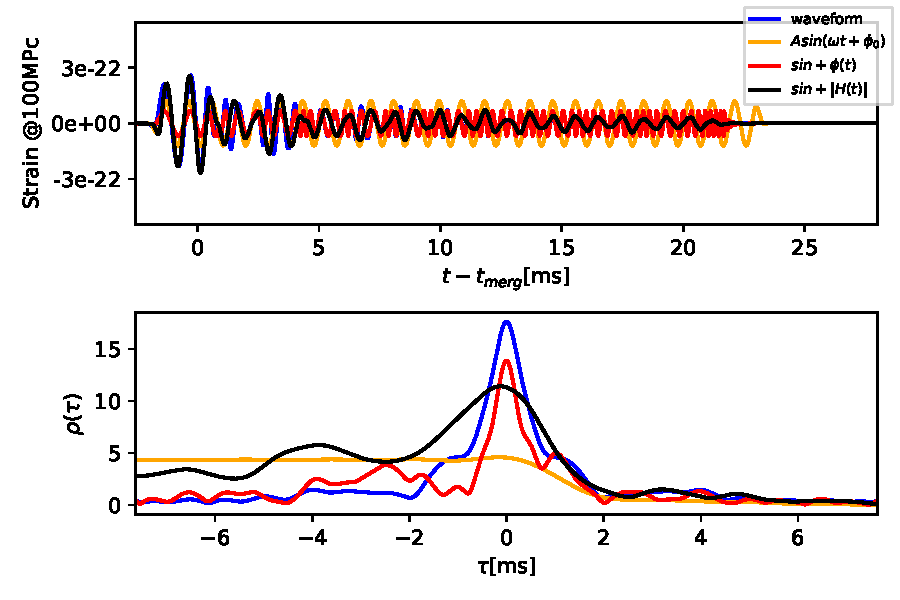
\includegraphics[width=0.6\textwidth, angle=0]{images/Data_analysis/results/phi-A0.pdf}
\caption{Waveform with a strange amplitude modulation from the CoRe catalog}
\label{analysis}
\end{center}
All models overlapped with the waveform BAM:0027(top), producing every single SNR curve as a function fo timeshift(bottom). Colors will be kept the same throughout the rest of the analysis; blue for the waveform(optimal), red for $\sin$ with phase evolution, black for the $\sin$ with amplitude evolution, and monochromatic in orange.
\end{figure}
\FloatBarrier

\subsection*{Findings}

\subsubsection*{Postmerger with rectangular windowing}

\begin{figure}[hbt!]
\begin{center}
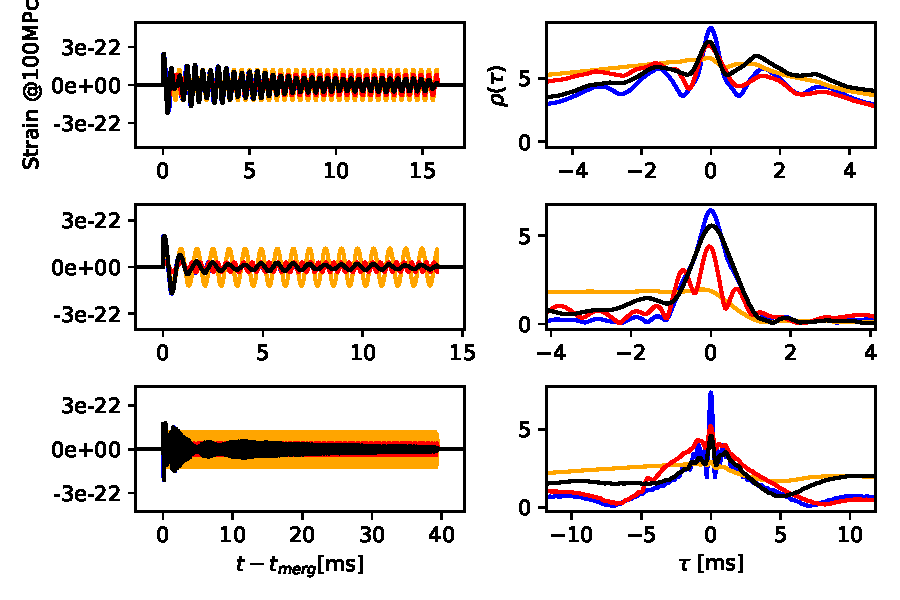
\includegraphics[width=0.7\textwidth, angle=0]{images/Data_analysis/results/phi-A1.pdf}
\caption{Partial modelling for $q=1$, $q>1.6$ and $\chi{eff}>0.2$ waveforms}
\end{center}
This image shows the time domain representations of all models(left), and their respective overlap as a function of timeshift(right). Colors follow the same pattern described in figure \ref{analysis}. The top waveform belongs to an equal mass system $q=1$, the one in the middle panel is a high mass ratio waveform $q>1.5$ and the lower panel shows a spining waveform$\chi_{eff}>0.2$.
\end{figure}

\begin{figure}[hbt!]
\begin{center}
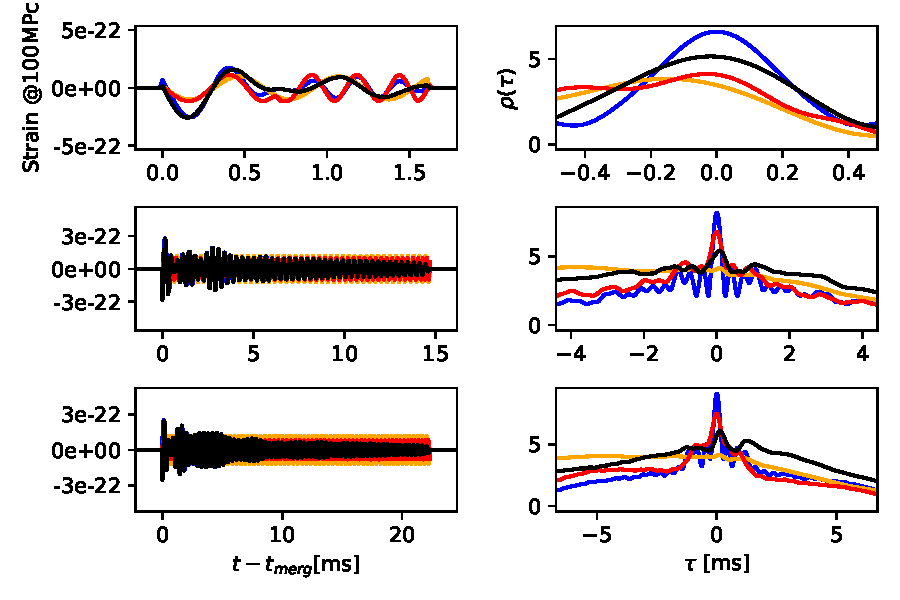
\includegraphics[width=0.7\textwidth, angle=0]{images/Data_analysis/results/phi-A2.pdf}
\caption{Partial modelling for $\delta>1.6$ , $e>0.4$, and $q=1$+viscuous hydrodynamics waveforms}
\end{center}
This image shows the time domain representations of all models(left), and their respective overlap as a function of timeshift(right). Colors follow the same pattern described in figure \ref{analysis}. The top waveform belongs to an heavy system $\delta>1.6$(see equation \ref{delta}), the one in the middle panel is a highly eccentric waveform $e>0.4$ and the lower panel shows a waveform with viscuous hydrodynamics.
\end{figure}
\FloatBarrier


In the case of eccentric and heavy mass waveforms, we see that a perfect amplitude evolution model would get 86\%  and 78\% of what a perfect model could get, regardless of the simple phase evolution modeling causing many misalignments in the late tail of the signal. On the other hand, equal mass systems and precessing systems would benefit much more from a very good phase evolution modeling. The inclusion of viscous hydrodynamics would not change this statement.


\begin{table}[!htbp]
\begin{center}

\begin{tabular}{ccccc}

simulation&$S_{opt}$&$\alpha(\phi_{const.})$&$\alpha(\phi(t))$&$\alpha(|H(t)|)$\\ 
\hline\\ 
$\mathrm{{q=1}_{_{_{(BAM:0035)}}}}$&8.943&0.734&0.841&0.875\\  
$\mathrm{{q>1.6}_{_{_{(BAM:0021)}}}}$&6.429&0.293&0.679&0.863\\  
$\mathrm{{X_{eff}>0.2}_{_{_{(BAM:0110)}}}}$&7.350&0.398&0.707&0.622\\  
$\mathrm{{\delta>1.6}_{_{_{(BAM:0011)}}}}$&6.607&0.535&0.611&0.778\\  
$\mathrm{{e>0.4}_{_{_{(BAM:0114)}}}}$&8.186&0.515&0.827&0.646\\  
$\mathrm{{visc.\hspace{1mm} HD}_{_{_{(THC:0019)}}}}$&9.122&0.461&0.819&0.638\\  
\hline\\ 

\end{tabular}
\end{center}
\caption{rectangular windowing. signal to noise ratio recovery for perfect phase and amplitude modelling.}
This table summarizes the results of the analysis for all models when introducing the hard cutoff mentioned in section X using the rectangular window to get the postmerger oscillations. It lists the amount of optimal SNR one could get with Einstein telescope at 100MPc, the third column tells how much SNR recovery had the monochromatic model, the fourth column for the model with phase evolution, and the fifth column for the monochormatic model with amplitude evolution.
\label{table untapered}
\end{table}
\FloatBarrier

\subsubsection*{Tapered postmerger: Impacts of spectral leakage}

It seems plausible to discuss whether the presence of the hard cutoff introduced by the rectangular window on the issues of the postmerger cause when computing FFTs and may affect the relative height of the peaks so that the maxima switch paces. This analysis will allow a few cycles before maximum amplitude and taper the signal using a Tukey window of parameter n.

\begin{figure}[hbt!]
\begin{center}
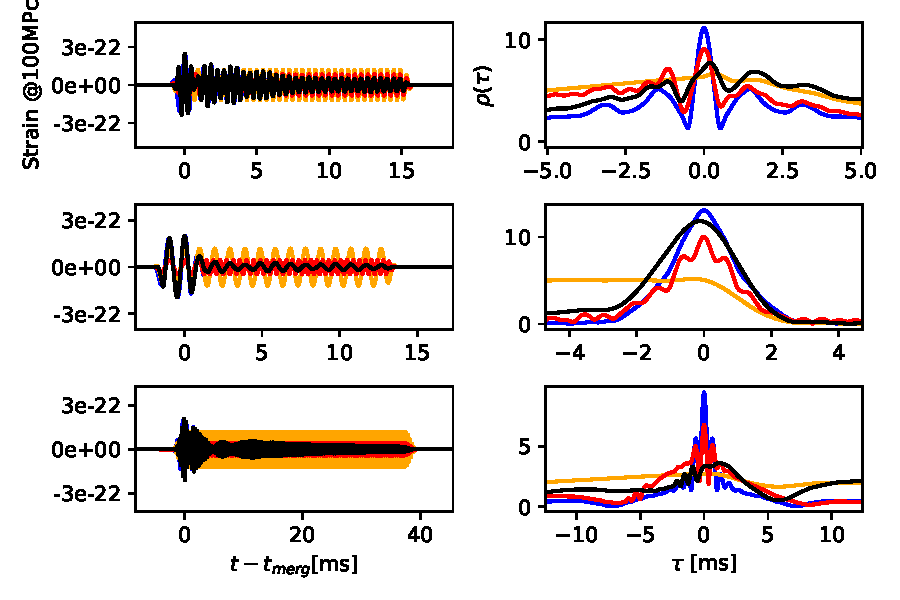
\includegraphics[width=0.7\textwidth, angle=0]{images/Data_analysis/results/phi-A3.pdf}
\caption{Tappered partial modelling for $q=1$, $q>1.6$ and $\chi{eff}>0.2$ waveforms}
\end{center}
This image shows the time domain representations of all models(left), and their respective overlap as a function of timeshift(right). Colors follow the same pattern described in figure \ref{analysis}. The top waveform belongs to an equal mass system $q=1$, the one in the middle panel is a high mass ratio waveform $q>1.5$ and the lower panel shows a spining waveform$\chi_{eff}>0.2$.
\end{figure}

\begin{figure}[hbt!]
\begin{center}
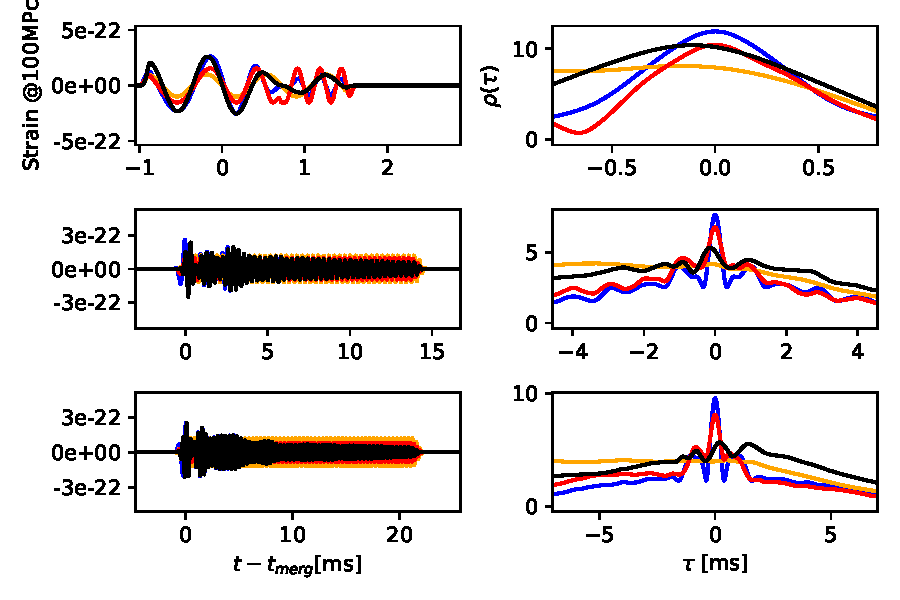
\includegraphics[width=0.7\textwidth, angle=0]{images/Data_analysis/results/phi-A4.pdf}
\caption{Tappered partial modelling for $\delta>1.6$ , $e>0.4$, and $q=1$+viscuous hydrodynamics waveforms}
\end{center}
This image shows the time domain representations of all models(left), and their respective overlap as a function of timeshift(right). Colors follow the same pattern described in figure \ref{analysis}. The top waveform belongs to an heavy system $\delta>1.6$(see equation \ref{delta}), the one in the middle panel is a highly eccentric waveform $e>0.4$ and the lower panel shows a waveform with viscuous hydrodynamics.
\end{figure}
\FloatBarrier

Results from tapered signals do not change the statement made for the hard cutoff case. However, instead emphasizes that phase modeling is most important for equal mass waveforms precessing waveforms and equal mass waveforms, including viscous HD. High mass ratio waveforms are still better recovered by the amplitude evolution model; however, phase evolution gets closer.


\begin{table}[!htbp]
\begin{center}

\begin{tabular}{ccccccc}
simulation&time before merger[ms]&n-tukey&$S_{opt}$&$\alpha(\phi_{const.})$&$\alpha(\phi(t))$&$\alpha(|H(t)|)$\\ 
\hline\\ 
$\mathrm{{q=1}_{_{_{(BAM:0035)}}}}$&1.0&0.1&11.132&0.596&0.815&0.654\\  
$\mathrm{{q>1.6}_{_{_{(BAM:0021)}}}}$&2.0&0.1&13.058&0.389&0.766&0.900\\  
$\mathrm{{X_{eff}>0.2}_{_{_{(BAM:0110)}}}}$&2.0&0.1&9.447&0.288&0.718&0.381\\  
$\mathrm{{\delta>1.6}_{_{_{(BAM:0011)}}}}$&1.0&0.1&11.904&0.666&0.876&0.856\\  
$\mathrm{{e>0.4}_{_{_{(BAM:0114)}}}}$&0.5&0.1&7.674&0.550&0.884&0.662\\  
$\mathrm{{visc.\hspace{1mm} HD}_{_{_{(THC:0019)}}}}$&1.0&0.1&9.570&0.436&0.848&0.577\\  
\hline\\ 
\end{tabular}

\end{center}
\caption{Effects of Tukey window. Signal to noise ratio recovery for perfect phase and amplitude modelling}
This table summarizes the results of the analysis for all models when tapering the waveform using a Tukey window to get the postmerger oscillations. It lists the  SNR  recovery results with Einstein telescope at 100MPc, the second column gives(roughly) the time before maximum amplitude(merger) that allowed the window,  the third column tells the Tukey parameter used and the last 4 columns represent the same kind of data shown in table \ref{table untapered}.
\end{table}
\FloatBarrier

\newpage
\addcontentsline{toc}{part}{Conclusions}

\chapter*{Conclusions}

Modeling the postmerger BNS GW signal is a very interesting open problem. Future detectors being much more sensitive in the kHz band will require the community to have calibrated phenomenological models for the whole BNS signal for the next decade. Future improvements on current phenomenological models and advances in universal and quasi-universal relations help reduce the number of parameters a model would require since they could be inferred from the inspiral or other observations.

This thesis explored the possibility of simple modeling on every waveform in available catalogs, and it complemented those results by addressing whether amplitude or phase evolution modeling could be prioritized separately depending on the source. 
 
The initial analysis showed how the finite monochromatic model performed well on equal mass waveforms and precessing waveforms with only one amplitude minimum. It recovered from 60 to 80\% of the optimal SNR because their waveforms do not have substantial variations in the phase or phase velocity nor significant amplitude variations that could account for phaseshifts of the order of $\pi$ radians. Some sources are above the imposed threshold for detection, and implementing a model with constant amplitude but better phase evolution would get more than 80\% of the SNR while recovering all the signal cycles.

Short waveforms with weighted frequencies around 3kHz belong to systems with $\delta=\frac{M}{M_{TOV}} > 1.6$. The simple monochromatic template model recovered from 80-98\% of the optimal SNR, being a reasonably good model for them. However, most of them are not loud enough to be detectable if they are generated by a source at a distance of 100MPc or more. Nevertheless, closer sources like GW170817 could have detectable postmerger phases by third-generation detectors.

High mass ratio and highly eccentric waveforms are the best candidates for detection at 100MPc or more. They feature a few loud oscillations after maximum amplitude that contain 60 to 95\% followed by a lower amplitude tail. The transition from the high amplitude initial part to the low amplitude tail looks pretty challenging to recover with a Monochromatic template model because the matched filtering algorithm would not gain much SNR by considering a longer wave. A better amplitude evolution would change this, significantly improving the SNR gains while recovering the low amplitude tail much better.


%Amplitude modeling is more important for short signals generated by systems with a total gravitational mass greater than 1.6  times the Maximum TOV mass and waveforms generated by systems with a high mass ratio greater than 1.6. On the other hand, signals generated by equal mass non-spinning binaries and spinning binaries with only one deep strain minimum in the time domain are already well recovered by a monochromatic signal. However, they would significantly improve if one provides a model with a much better phase evolution.




 







